\documentclass{article}
\usepackage{graphicx}
\usepackage{amsmath, amsthm, amssymb}
\usepackage{multicol}
\usepackage[utf8]{inputenc}
\usepackage{enumerate} 
\usepackage{lmodern,microtype}
\usepackage{hyperref}
\usepackage{polski}
\usepackage{graphicx}
\usepackage{float}
\usepackage{listings}

\author{Matylda Mordal}
\title{\textbf{Lista 2 sprawozdanie}}
\date{}

\begin{document}
	\maketitle
	
	\section*{Zadanie 1}
	
	\begin{lstlisting}[language=C++, tabsize=3]
	int PARTITION(int A[], int p, int r) {
		int x = A[r];   
		int i = p - 1;   
		
		for (int j = p; j <= r - 1; j++) {
			if (A[j] <= x) {     
				i++;             
				swap(A[i], A[j]); 
			}
		}
		swap(A[i + 1], A[r]); 
		return i + 1; 
	}
	\end{lstlisting}
	
	Funkcja PARTITION potrzebna jest do algorytmu QUICK\_SORT, dzieli ona tablice wokół elementu zwanego pivotem.
	\begin{itemize}
		\item Ustawienie pivota: Pivotem jest ostatni element podtablicy, czyli x = A[r].
		
		\item Inicjalizacja wskaźnika i:
		Wskaźnik i początkowo wskazuje na "granice" elementów mniejszych lub równych pivotowi. Jest ustawiany na p - 1, czyli na pozycję przed początkiem podtablicy.
		
		\item Iteracja po elementach podtablicy:
		Pętla for przechodzi przez wszystkie elementy od p do r-1:
		Jeśli bieżący element A[j] jest mniejszy lub równy pivotowi, zwiększa się wskaźnik i i następuje zamiana elementu A[j] z A[i].
		To przesuwa element A[j] do strefy "mniejszych lub równych pivotowi".
		
		\item Umieszczenie pivota na właściwej pozycji:
		Po zakończeniu pętli pivot (czyli A[r]) zostaje zamieniony z elementem A[i+1]. Dzięki temu pivot trafia na swoją ostateczną, posortowaną pozycję.
		
		\item Zwracanie indeksu:
		Funkcja zwraca indeks i + 1, czyli pozycję, na której znajduje się pivot.
	\end{itemize}
	
	\begin{lstlisting}[language=C++, tabsize=3]
	void QUICK_SORT(double A[], int p, int r) {
		if (p < r) { 
			int q = PARTITION(A, p, r); 
			QUICK_SORT(A, p, q - 1);     
			QUICK_SORT(A, q + 1, r); 
		}
	}
	\end{lstlisting}
	
	Algorytm QUICK\_SORT to jeden z najszybszych i najczęściej używanych algorytmów sortowania. Działa w oparciu o strategię dziel i zwyciężaj .
	\begin{itemize}
		\item Warunek zakończenia rekurencji:
		Jeśli $p >= r$ (indeks początkowy jest większy lub równy indeksowi końcowemu), oznacza to, że podtablica ma jeden element lub jest pusta. W takim przypadku jest już posortowana, i algorytm kończy działanie dla tego zakresu.
		
		\item Podział tablicy:
		Wywoływana jest funkcja PARTITION, któram zwraca indeks q, pod którym znajduje się pivot w swojej posortowanej pozycji.
		
		\item Rekurencja:
		Funkcja QUICK\_SORT jest wywoływana osobno dla dwóch części:
		Dla lewej podtablicy: A[p..q-1].
		Dla prawej podtablicy: A[q+1..r].
	\end{itemize}
	
	\begin{figure}[H]
		\centering
		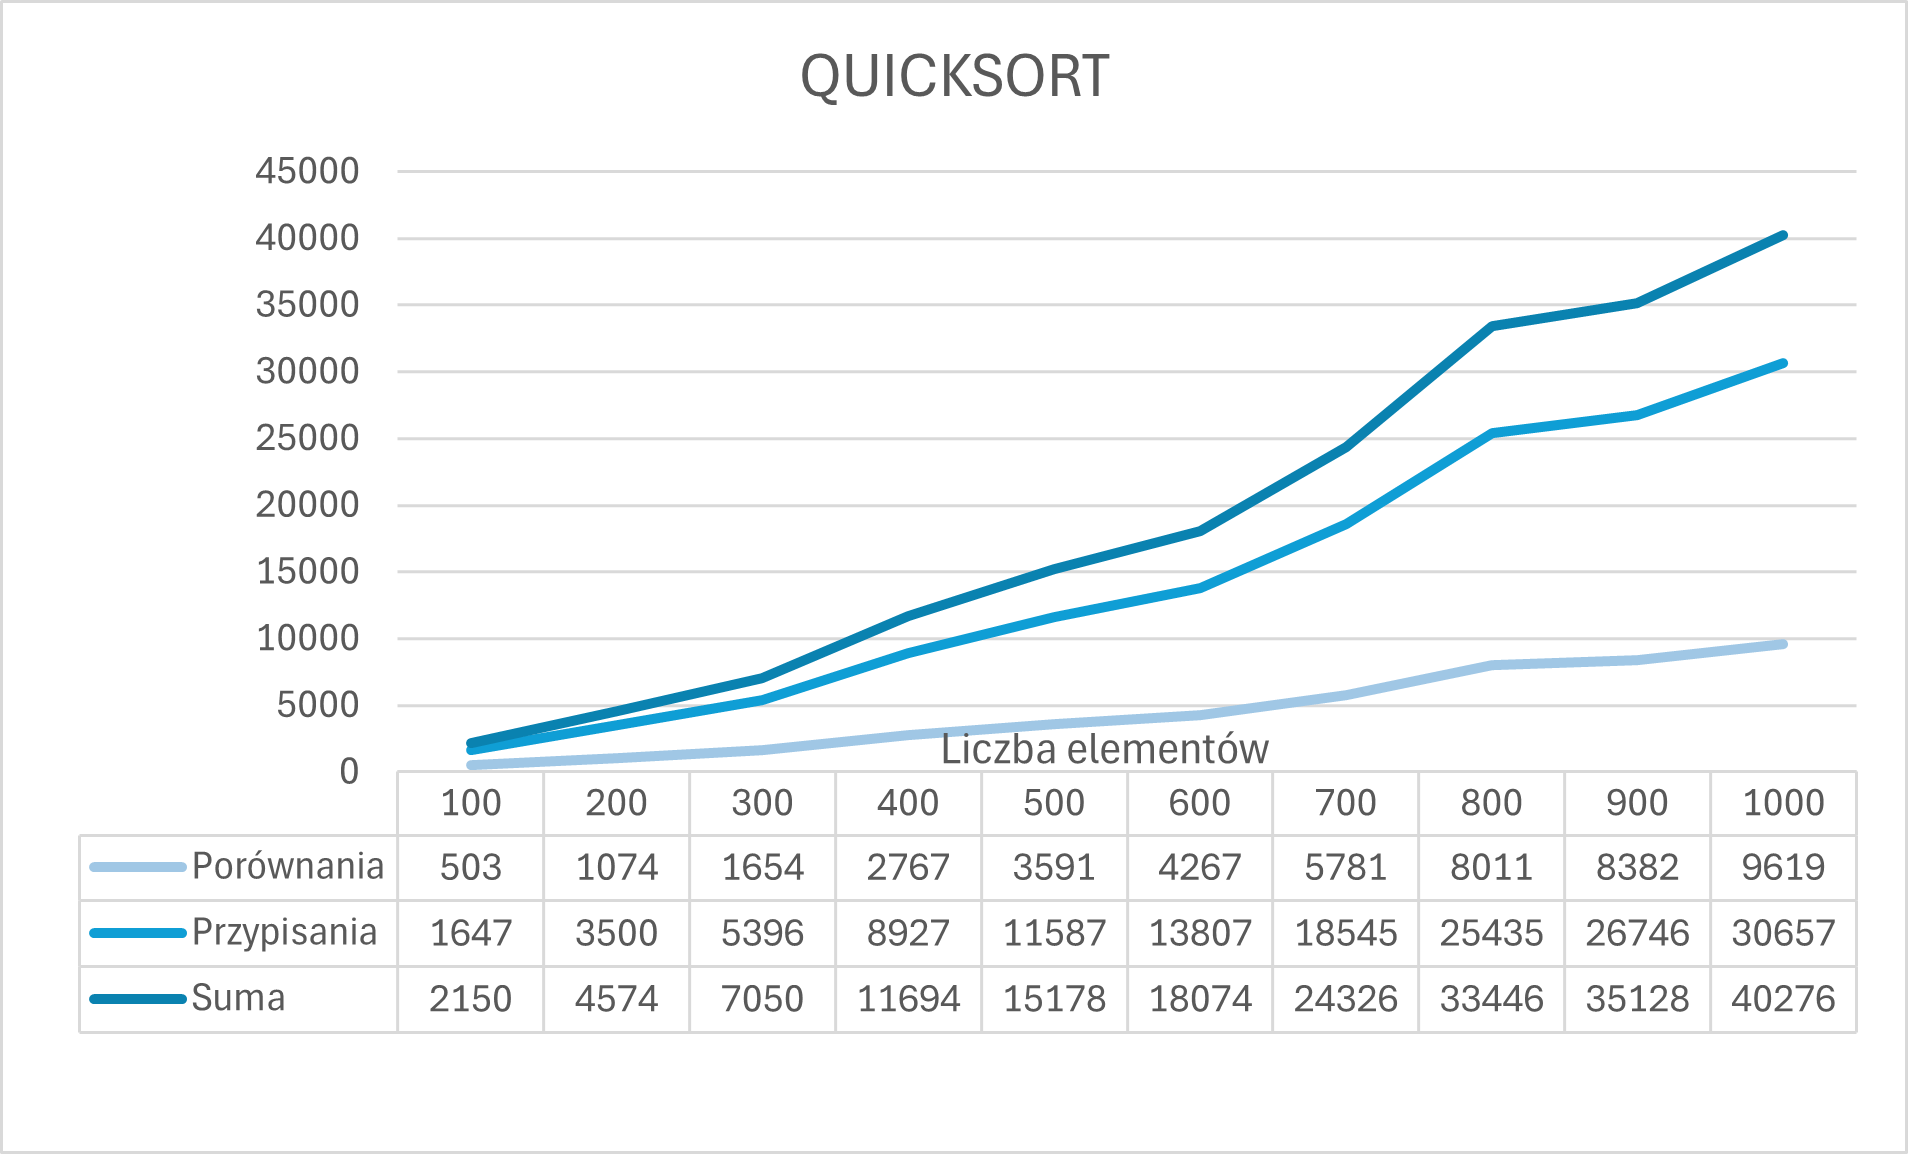
\includegraphics[width=0.9\textwidth]{QS11.png}
		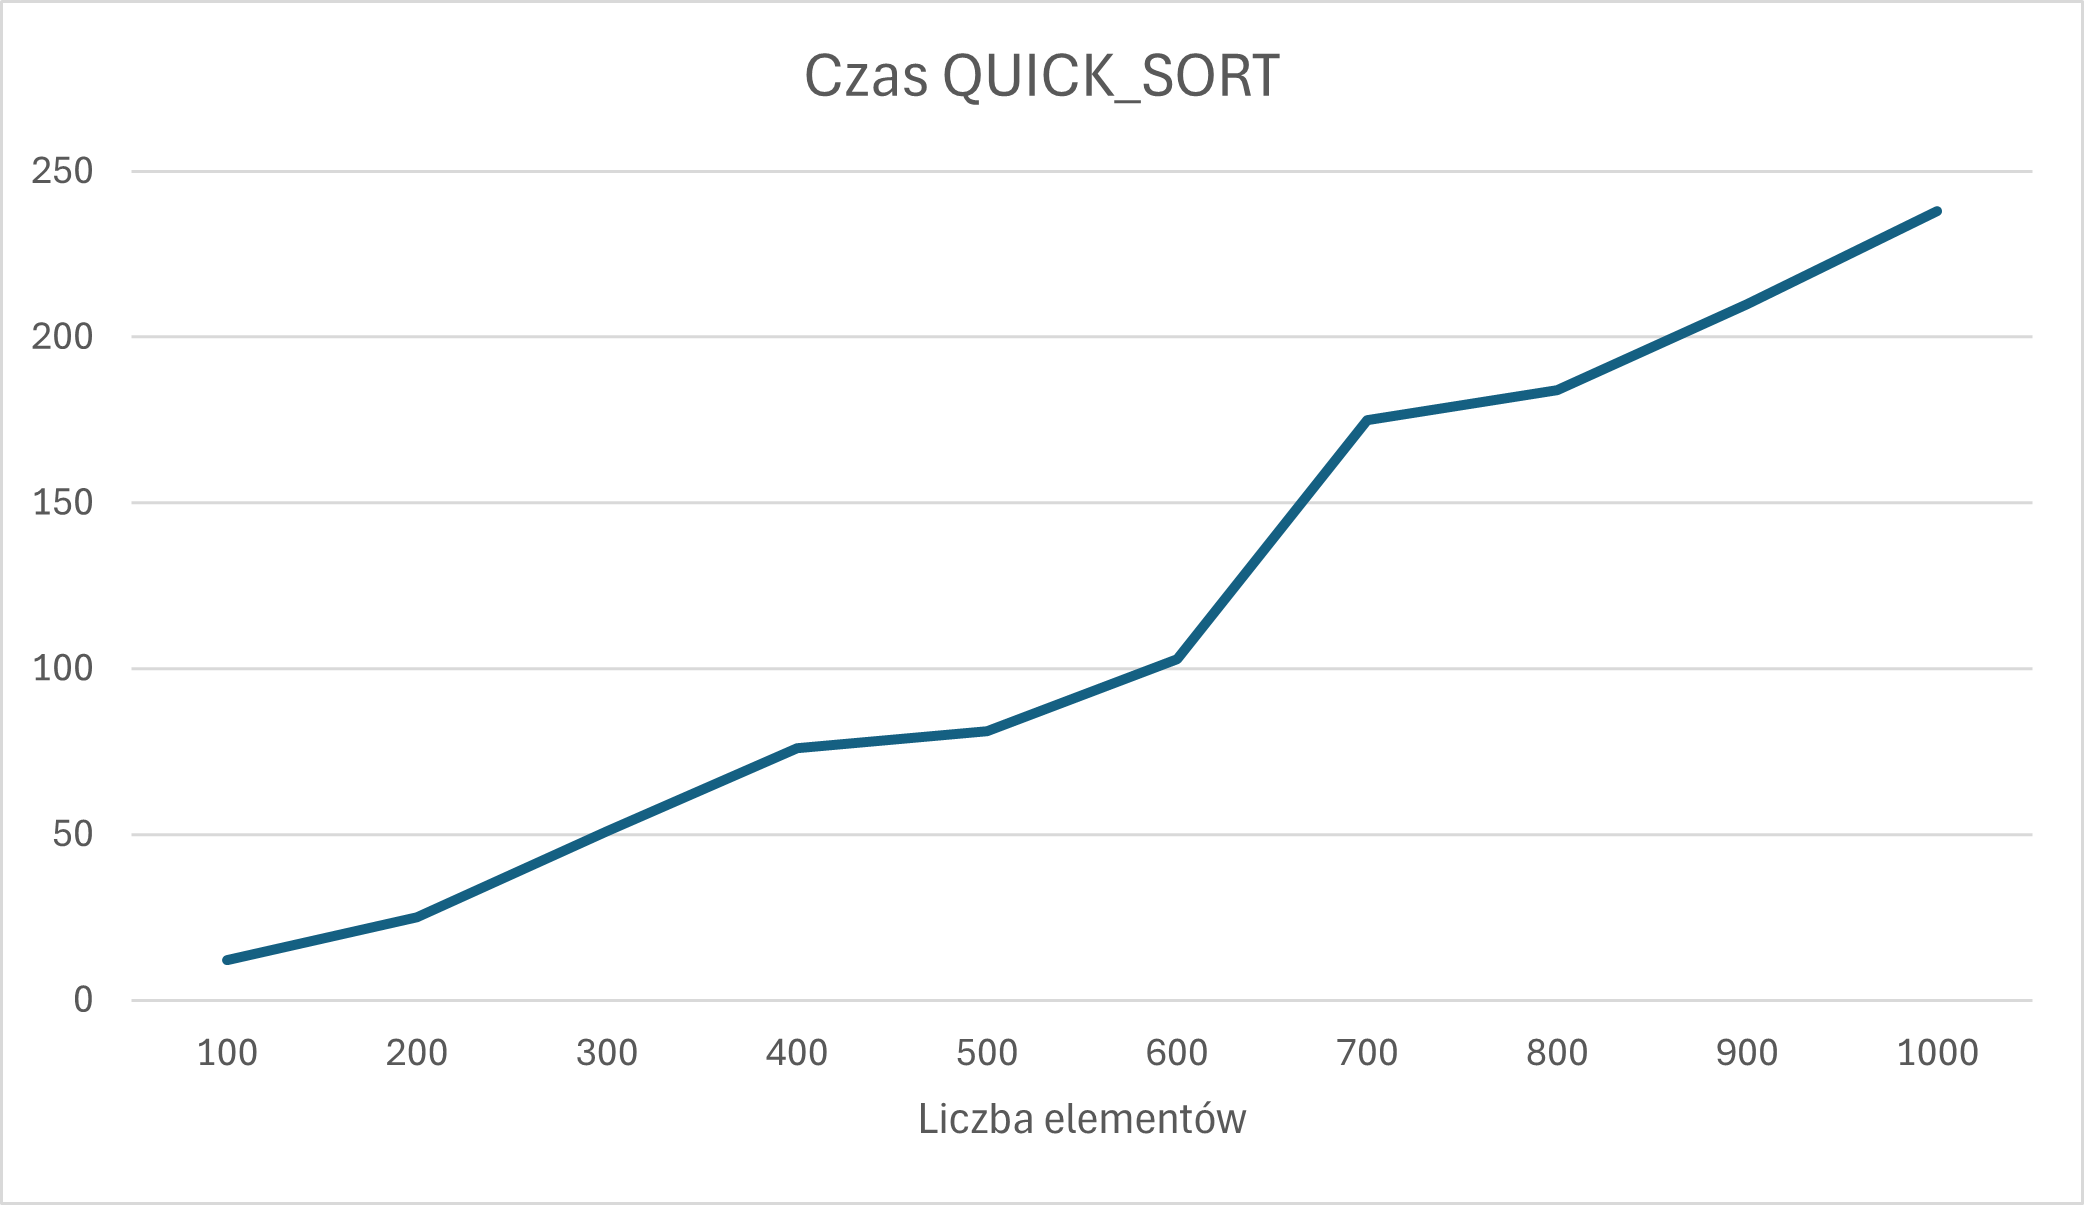
\includegraphics[width=0.9\textwidth]{QS12.png}
	\end{figure}
	
	\textbf{Porównania i przypisania:} Liczba porównań i przypisań rośnie mniej więcej liniowo lub kwadratowo wraz ze wzrostem liczby elementów. Jest to zgodne z teoretyczną złożonością QuickSorta:
	\begin{itemize}
		\item w najlepszym przypadku \(O(n \log n)\),
		\item w najgorszym przypadku \(O(n^2)\).
	\end{itemize}
	\textbf{Teoretyczna zgodność:} Wyniki potwierdzają teoretyczne założenia QuickSorta, czyli średnią złożoność obliczeniową \(O(n \log n)\).
	
	
	\begin{lstlisting}[language=C++, tabsize=3]
	void PARTITION2(double A[], int p, int r, int &x, int &y) {
		if (A[p] > A[r]) {
			std::swap(A[p], A[r]);
		}
		int pivot1 = A[p];
		int pivot2 = A[r];
		
		int i = p + 1;
		int a = p + 1; 
		int b = r - 1; 
		
		while (i <= b) {
			if (A[i] < pivot1) {
				swap(A[i], A[a]);
				a++;
			} else if (A[i] > pivot2) {
				swap(A[i], A[b]);
				b--;
				i--; 
			}
			i++;
		}
		
		a--;
		b++;
		swap(A[p], A[a]);
		swap(A[r], A[b]);
		
		x = a;
		y = b;
	}
	\end{lstlisting}
	
	Funkcja PARTITION2 implementuje algorytm podziału tablicy z dwoma pivotami w kontekście sortowania.
	\begin{itemize}
		\item Porównanie i zamiana pivotów:
		Na początku funkcja sprawdza, czy pierwszy element tablicy (A[p]) jest większy od ostatniego (A[r]). Jeśli tak, zamienia je miejscami. 
		
		\item Przypisanie pivotów:
		pivot1 = A[p]: Mniejszy pivot.
		pivot2 = A[r]: Większy pivot.
		
		\item Przypisanie zmiennych:
		i = p + 1: Indeks aktualnego elementu.
		a = p + 1: Indeks granicy elementów mniejszych od pivot1.
		b = r - 1: Indeks granicy elementów większych od pivot2.
		
		\item Podział tablicy:
		Pętla przechodzi przez każdy element pomiędzy \(p+1\) a \(r-1\):
		\begin{itemize}
			\item Jeśli $A[i] < pivot1$ :
			Zamienia miejscami A[i] i A[a].
			\(a\) jest zwiększany.
			\item Jeśli $A[i] > pivot2$ :
			Zamienia miejscami A[i] i A[b].
			\(b\) jest zwiększany.
			\(i\) jest zmniejszany, aby ponownie sprawdzić przestawiony element.
			\item W przeciwnym wypadku element pozostaje w strefie elementów pomiędzy pivotami.
		\end{itemize}
		Po każdej iteracji \(i\) jest zwiększane.
		
		\item Ostateczne umiejscowienie pivotów:
		Zamiana mniejszego pivotu z elementem na granicy elementów mniejszych (A[a]).
		Zamiana większego pivotu z elementem na granicy elementów większych (A[b]).
		Zwracanie pozycji pivotów:
		x = pozycja mniejszego pivotu.
		y = pozycja większego pivotu.
	\end{itemize}
	
	\begin{lstlisting}[language=C++, tabsize=3]
	void QUICK_SORT2(double A[], int p, int r) {
		if (p < r) {
			int x, y; 
			PARTITION2(A, p, r, x, y);
			
			QUICK_SORT2(A, p, x - 1);
			QUICK_SORT2(A, x + 1, y - 1);
			QUICK_SORT2(A, y + 1, r);
		}
			
		\end{lstlisting}
		
		Działanie funkcji QUICK\_SORT2:
		\begin{itemize}
			\item Warunek zakończenia rekurencji:
			Jeśli $p >= r$ (indeks początkowy jest większy lub równy indeksowi końcowemu), oznacza to, że podtablica ma jeden element lub jest pusta. W takim przypadku jest już posortowana, i algorytm kończy działanie dla tego zakresu.
			
			\item Podział tablicy:
			Wywoływana jest funkcja PARTITION2, która zwraca \(x\) i \(y\), w których znajdują się odpowiednio miejsca dla pivotów (pivot1 i pivot2).
			
			\item Rekurencja:
			Funkcja następnie wywołuje rekurencyjnie sortowanie dla trzech części:
			
			\begin{itemize}
				\item Pierwsza część: sortuje przedział od \(p\) do \(x-1\), który zawiera elementy mniejsze od pivot1.
				\item Druga część: sortuje przedział od \(x+1\) do \(y-1\), który zawiera elementy pomiędzy pivot1 a pivot2.
				\item Trzecia część: sortuje przedział od \(y+1\) do \(r\), który zawiera elementy większe od pivot2.
			\end{itemize}	
		\end{itemize}	
		
		\begin{figure}[H]
			\centering
			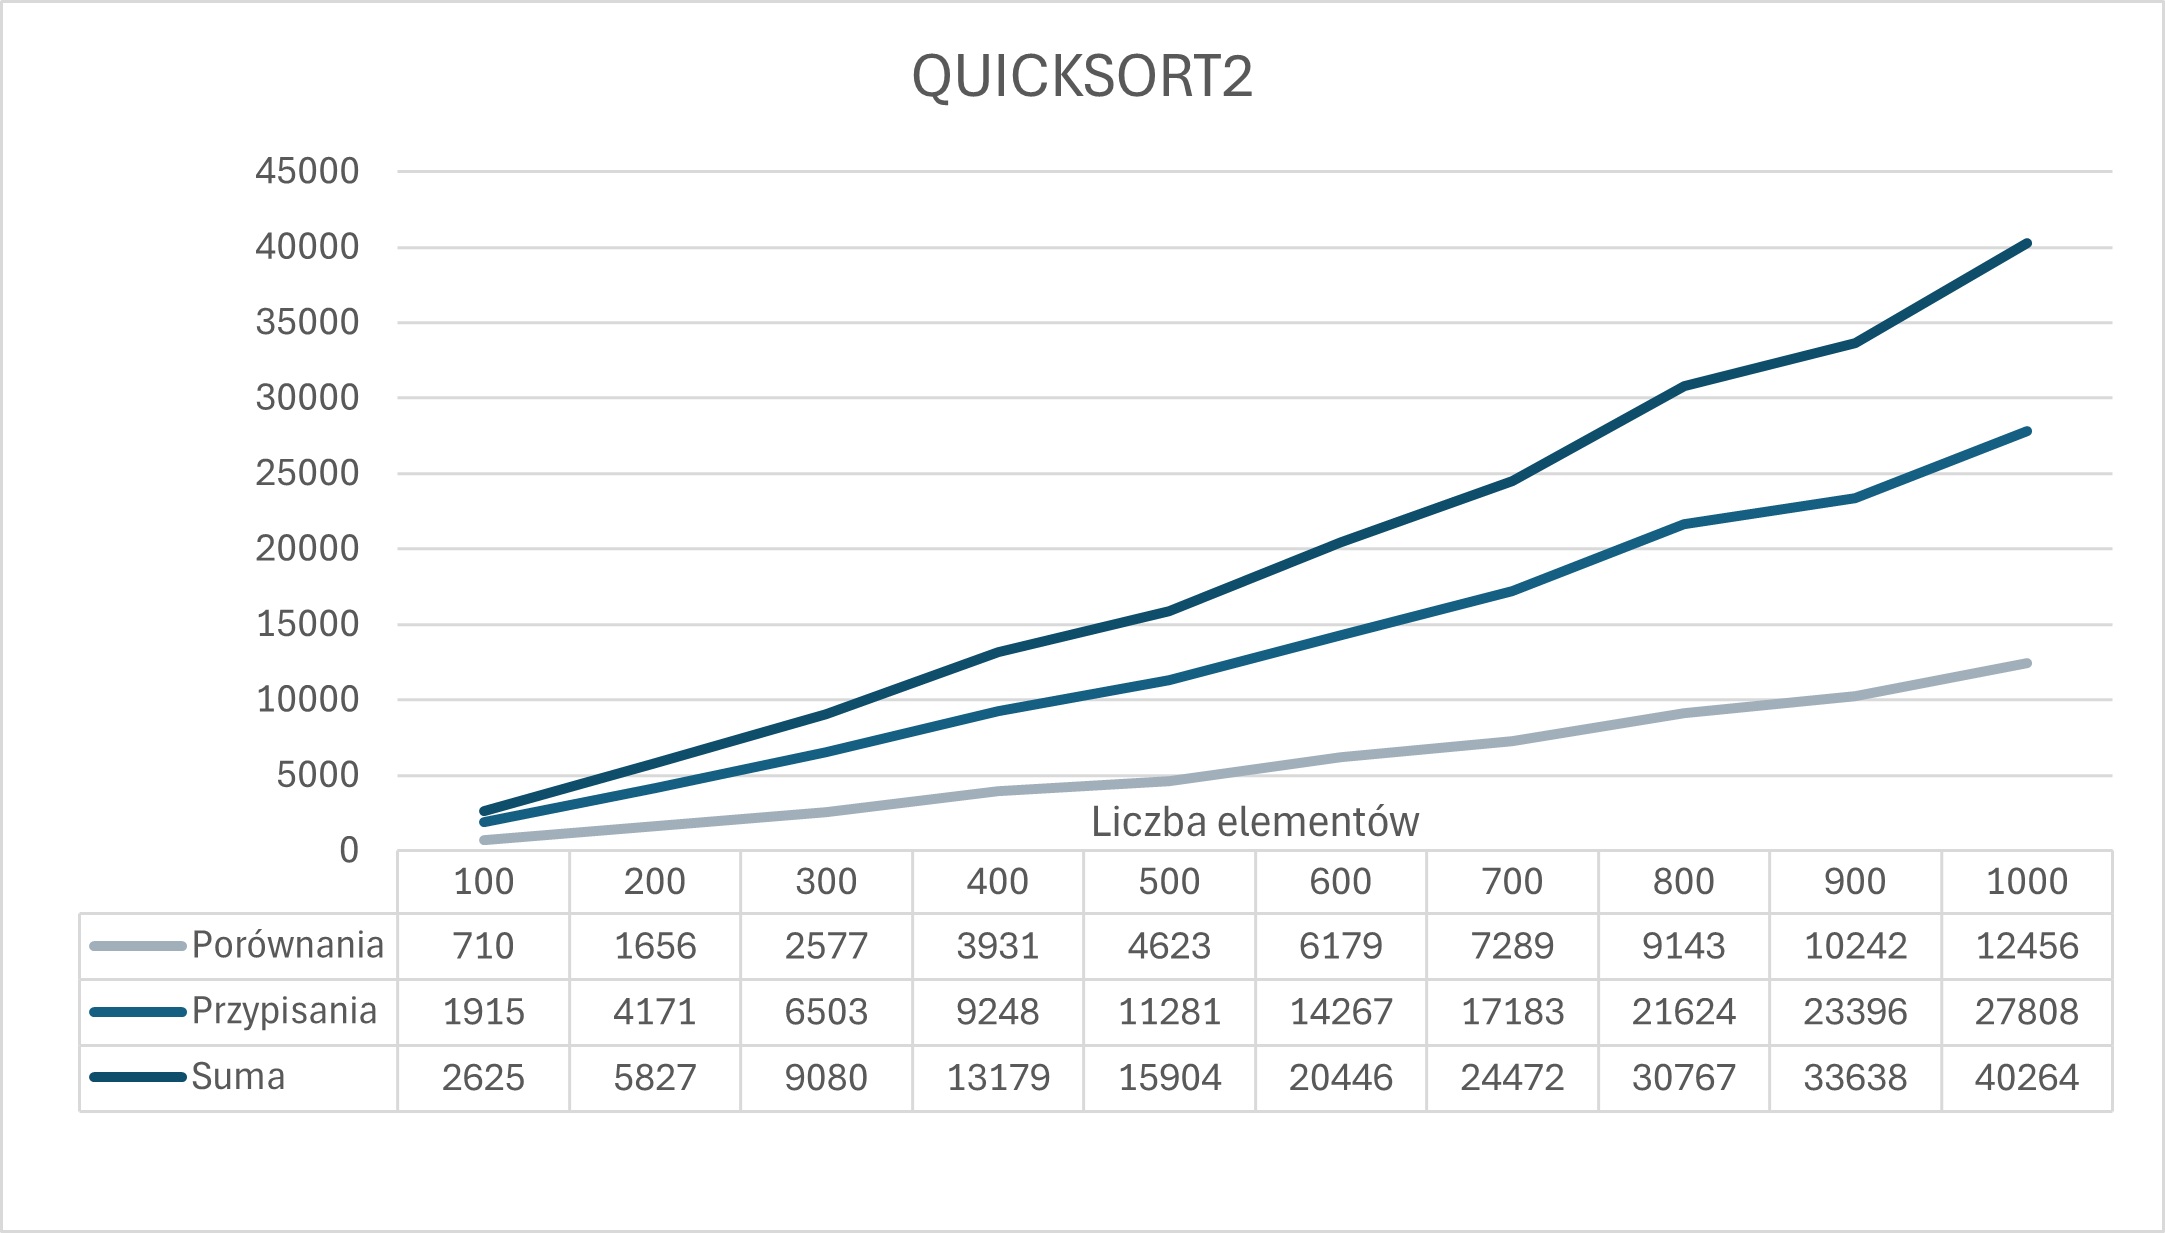
\includegraphics[width=0.9\textwidth]{QS21.png}
			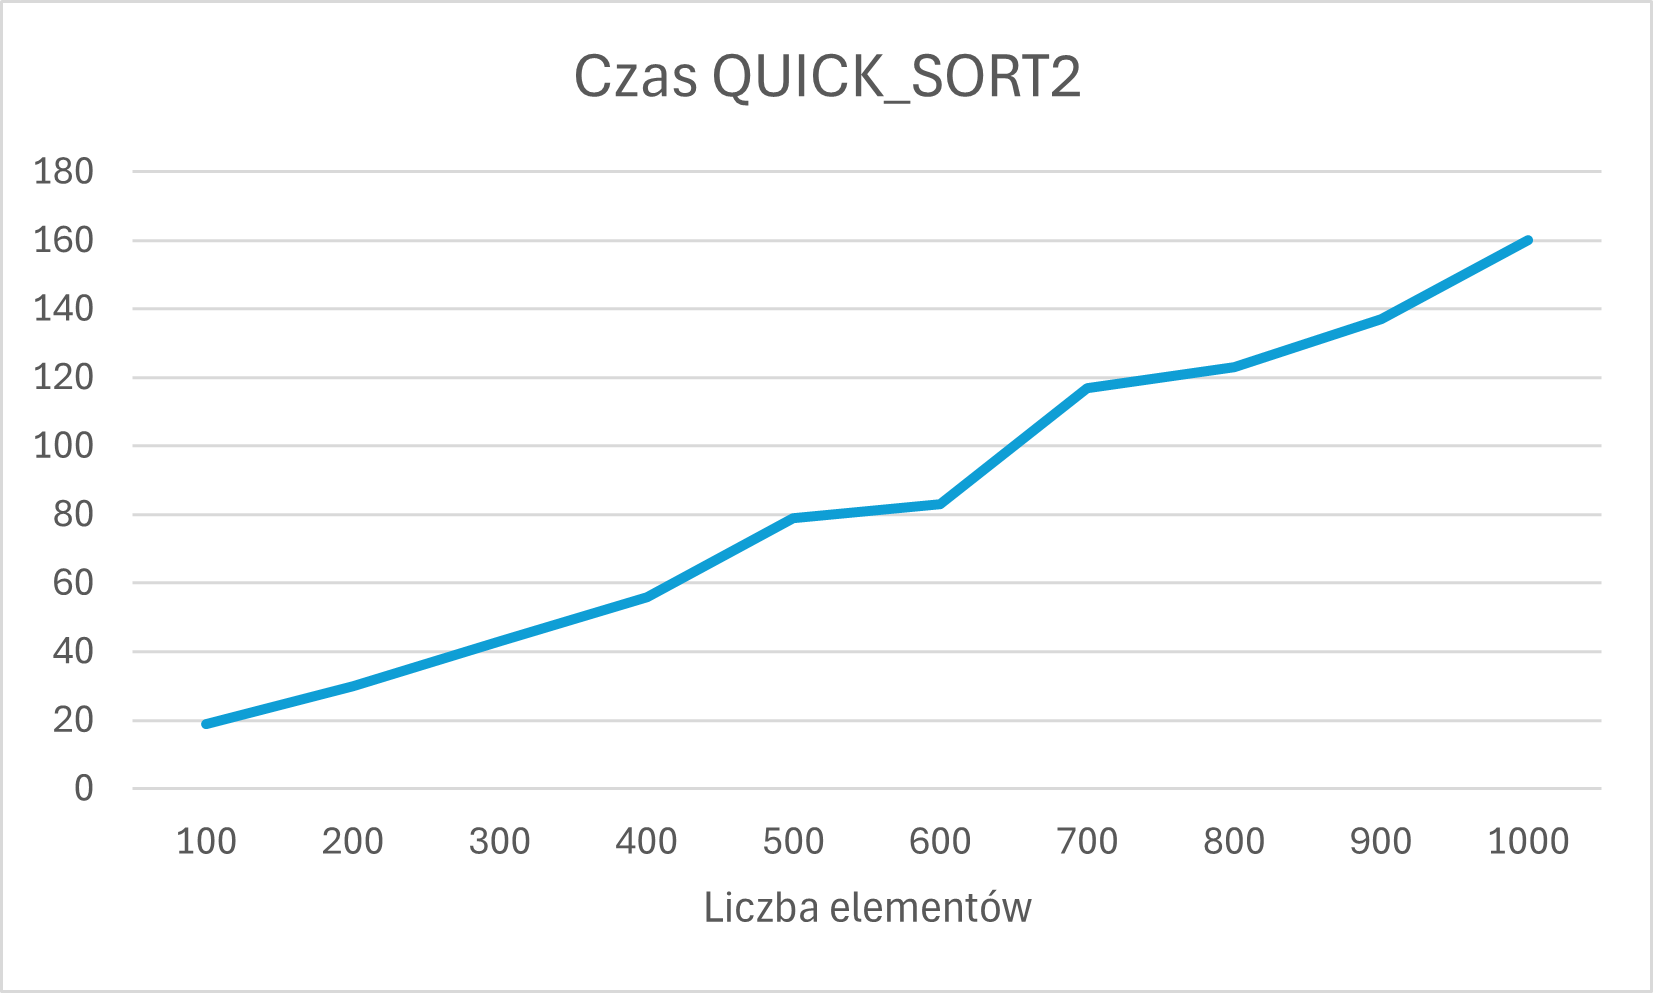
\includegraphics[width=0.9\textwidth]{QS22.png}
		\end{figure}
		
		\textbf{Porównania i przypisania} zwiększają się niemal liniowo w miarę wzrostu liczby elementów. \\
		Wraz ze wzrostem liczby elementów, liczba operacji (porównań i przypisań) rośnie szybciej niż liniowo, co sugeruje złożoność czasową zbliżoną do \( O(n \log n) \), ale z pewnym kosztem dodatkowym wynikającym z obsługi dwóch pivotów.\\
		Wzrost \textbf{czasu} jest bliski liniowej zależności od liczby elementów, co sugeruje, że implementacja jest dobrze zoptymalizowana. \\
		Klasyczny QuickSort zazwyczaj wymaga około \( O(n \log n) \) porównań i operacji, a QuickSort2 wydaje się osiągać podobny wynik, ale z większą liczbą przypisań, co wynika z bardziej złożonego procesu dzielenia tablicy.
		
		\newpage
		\section*{Zadanie 2}
		
		\begin{lstlisting}[language=C++, tabsize=3]
	void COUNTINGSORT(int A[], int n, int exp, int d) {
		int B[n];        
		int C[d] = {0};  
		
		for (int i = 0; i < n; i++) {
			int j = (A[i] / exp) % d;
			C[j]++;
		}
		
		for (int i = 1; i < d; i++) {
			C[i] += C[i - 1];
		}
		
		for (int i = n - 1; i >= 0; i--) {
			int j = (A[i] / exp) % d;
			B[C[j] - 1] = A[i];
			C[j]--;
		}
		
		for (int i = 0; i < n; i++) {
			A[i] = B[i];
		}
	}
		\end{lstlisting}
		
		Działanie funkcji COUNTINGSORT:
		\begin{itemize}
			\item Tworzenie pomocniczych tablic:
			B[n]: Tablica wynikowa, która będzie zawierać posortowane liczby.
			C[d]: Tablica zliczająca wystąpienia każdej wartości na danej pozycji 
			
			\item Zliczanie wystąpień dla danej cyfry:
			
			Dla każdej liczby w tablicy A[], wyciągana jest cyfra na pozycji zależnej od exp . Cyfra ta jest obliczana przez $(A[i] \div \text{exp}) \mod d$  , gdzie \(i\) to indeks w tablicy.
			Tablica C[] na końcu zawiera liczbę wystąpień każdej wartości w danym miejscu.
			
			\item Przekształcanie tablicy C[] na tablicę sum:
			Zaczynając od indeksu 1, do każdego elementu w tablicy C[] dodawana jest wartość poprzedniego elementu.
			Dzięki temu C[i] zawiera informację o liczbie elementów mniejszych lub równych i na danej pozycji. Ta operacja przekształca tablicę z liczby wystąpień na liczbę pozycji, na których powinny znaleźć się odpowiednie elementy w tablicy wynikowej B[].
			
			\item Tworzenie tablicy wynikowej B[]:
			Rozpoczynamy iterację przez tablicę A[] od końca. Jest to ważne, aby nie zmieniać kolejności elementów, które mają tę samą cyfrę na danej pozycji.
			Dla każdego elementu w A[], wyliczamy jego cyfrę na danej pozycji, a następnie umieszczamy ten element w odpowiednim miejscu w tablicy B[] zgodnie z liczbą wystąpień w tablicy C[]. Po umieszczeniu elementu, zmniejszamy wartość w C[], aby odpowiednio wskazać kolejne dostępne miejsce.
			
			\item Na końcu, po posortowaniu liczb na danej pozycji, zawartość tablicy B[] jest kopiowana do tablicy A[], aby tablica A[] zawierała teraz posortowane liczby.
		\end{itemize}
		
		\begin{lstlisting}[language=C++, tabsize=3]
	void RADIX_SORT(int A[], int n, int d, int k) {
		for (int i = 0, exp = 1; i < k; i++, exp *= d) {
			COUNTINGSORT(A, n, exp, d);
		}
	}
		\end{lstlisting}
		
		Działanie funkcji RADIX\_SORT:
		\begin{itemize}
			\item Zmienna exp reprezentuje wykładnik, który określa, na jaką pozycję wartości będziemy sortować w tej iteracji. Rozpoczynamy od exp = 1 , a w każdej kolejnej iteracji exp będzie mnożone przez d, aby przechodzić na kolejne pozycje wartości.
			
			\item Funkcja wykonuje pętlę for o k iteracjach. k to liczba wartości, więc w każdej iteracji sortujemy liczby według jednej pozycji.
			W każdej iteracji zmienia się wykładnik exp, który wskazuje, którą wartość w liczbach będziemy analizować.
			
			\item W każdej iteracji, dla danej pozycji wartości (określonej przez exp), wywoływana jest funkcja COUNTINGSORT, która sortuje liczby w tablicy A[] na podstawie tej konkretnej wartości.
			
			\item W każdej iteracji pętli exp jest mnożone przez d, co powoduje, że w kolejnej iteracji funkcja COUNTINGSORT będzie sortować liczby według następnej wartości.
			
			\item Proces jest powtarzany k razy. Po wykonaniu tych wszystkich iteracji tablica A[] jest posortowana. 
		\end{itemize}
		
		\begin{figure}[H]
			\centering
			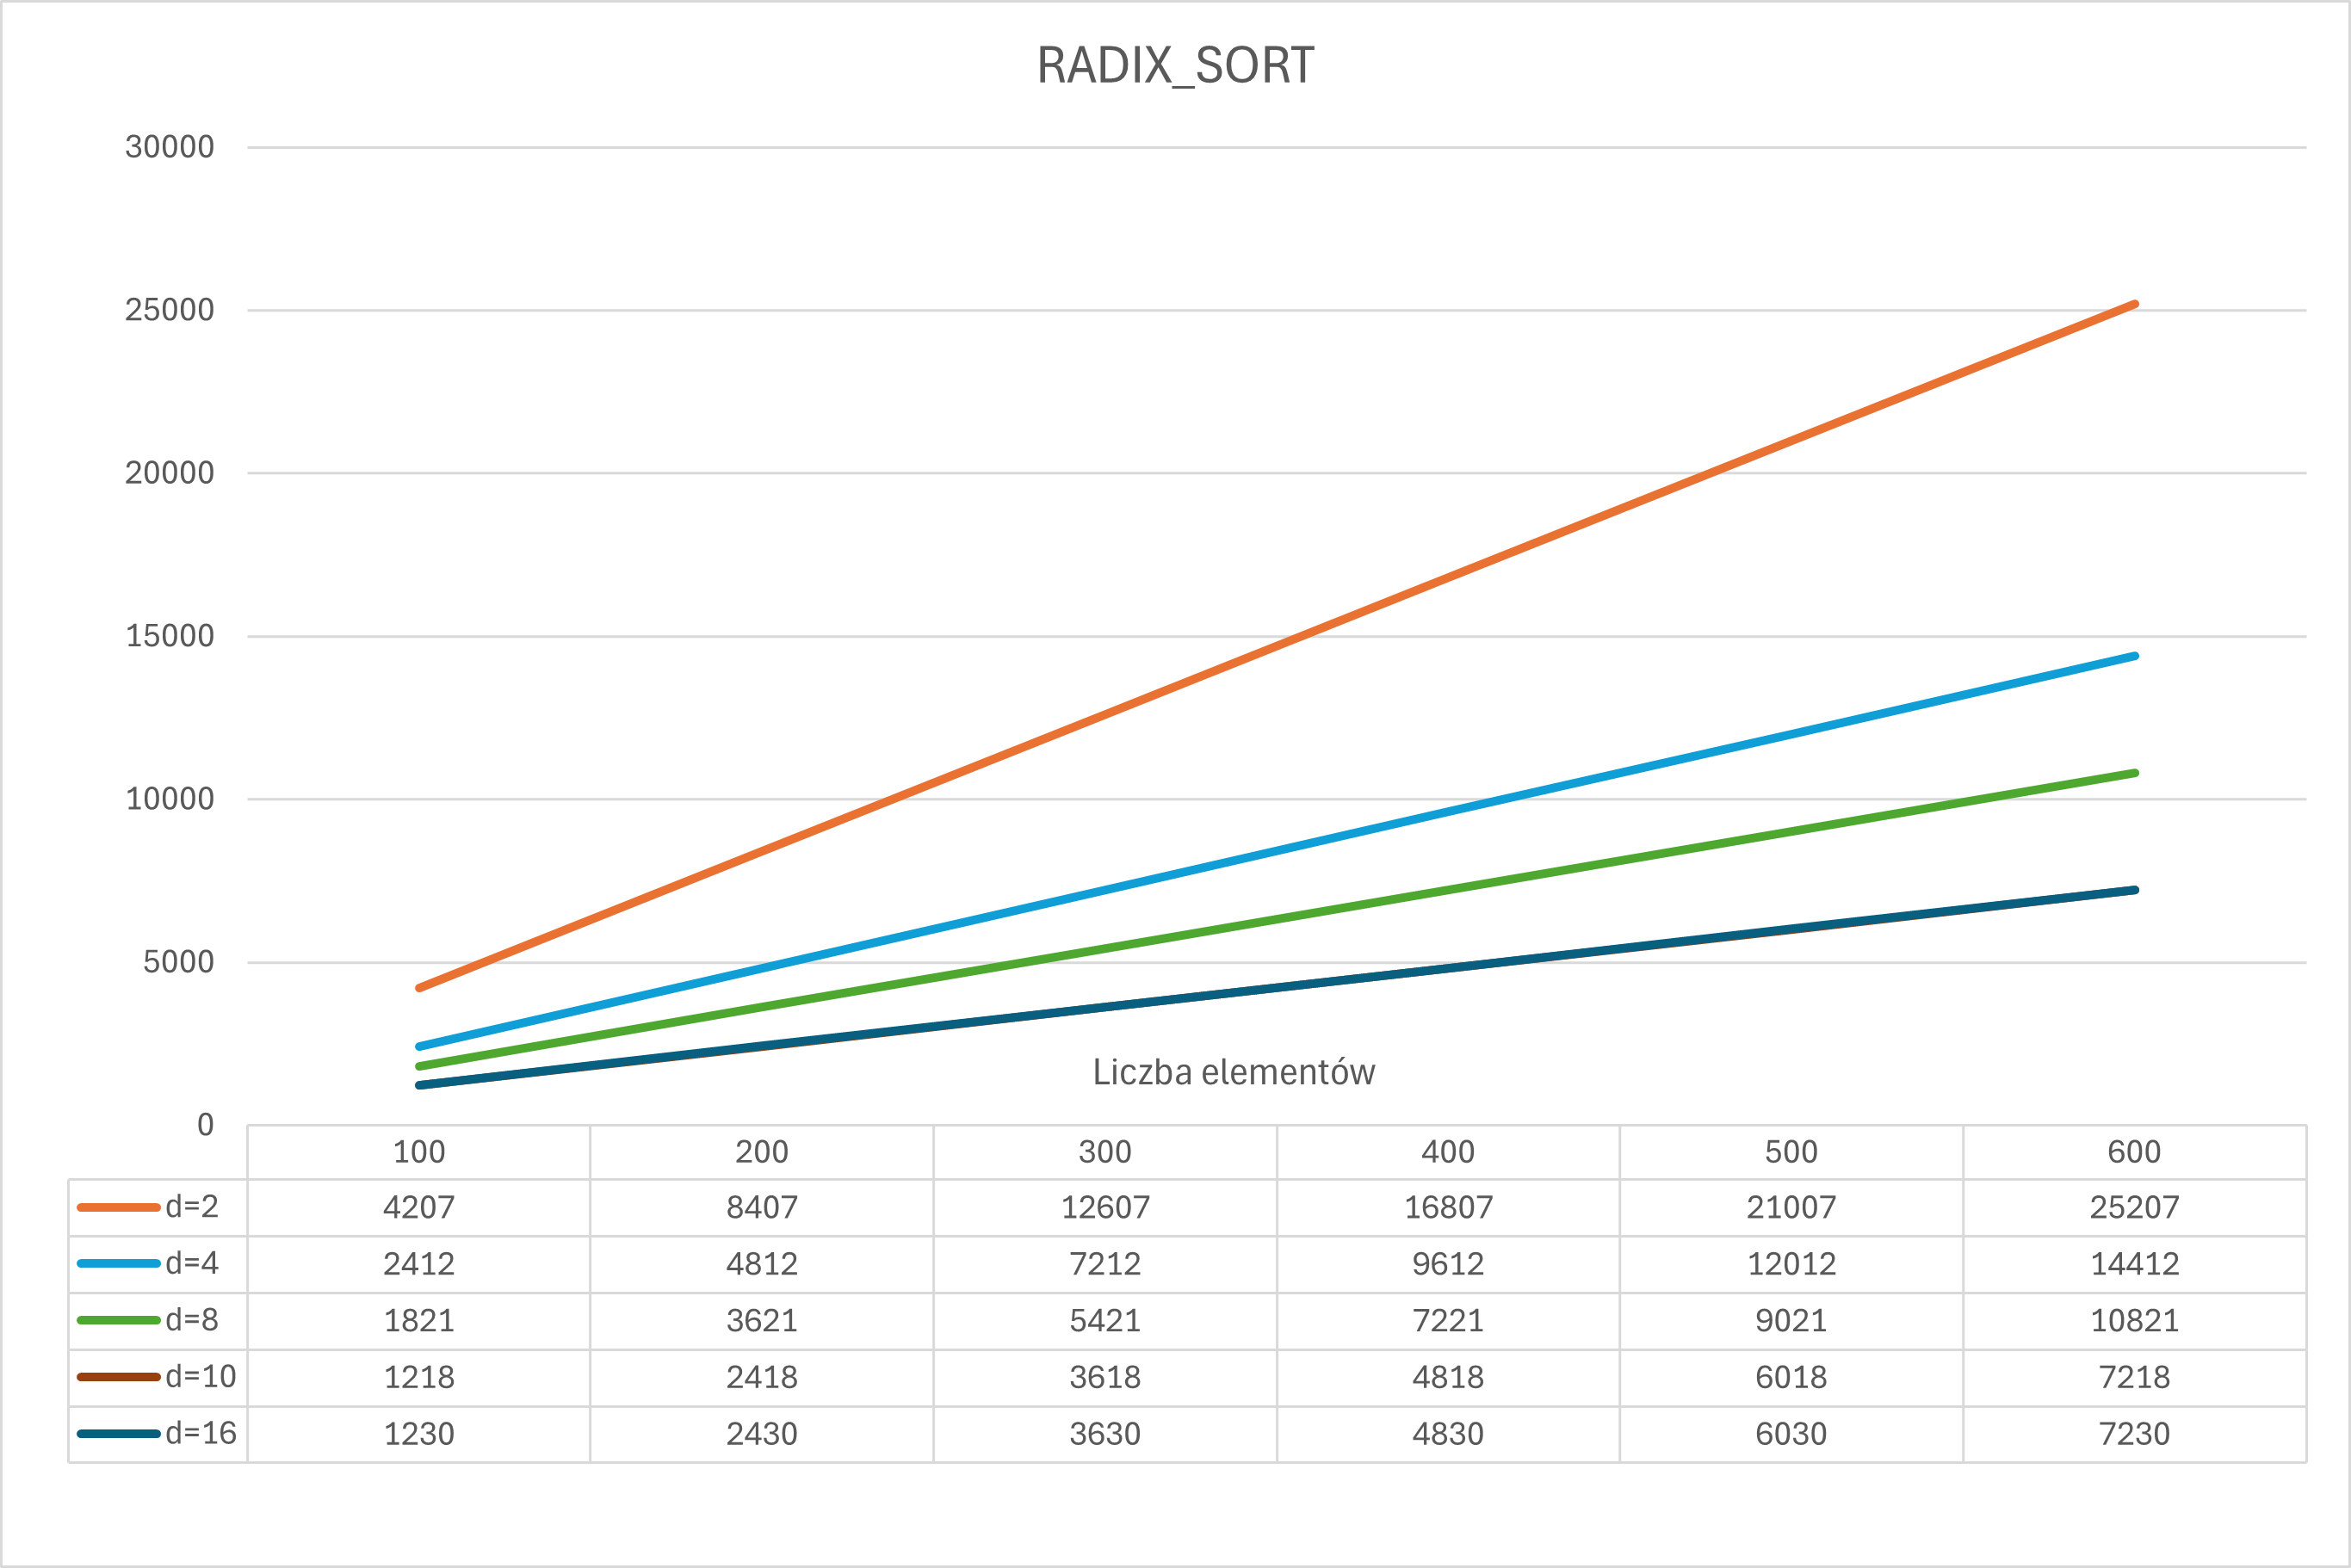
\includegraphics[width=0.9\textwidth]{RS11.png}
			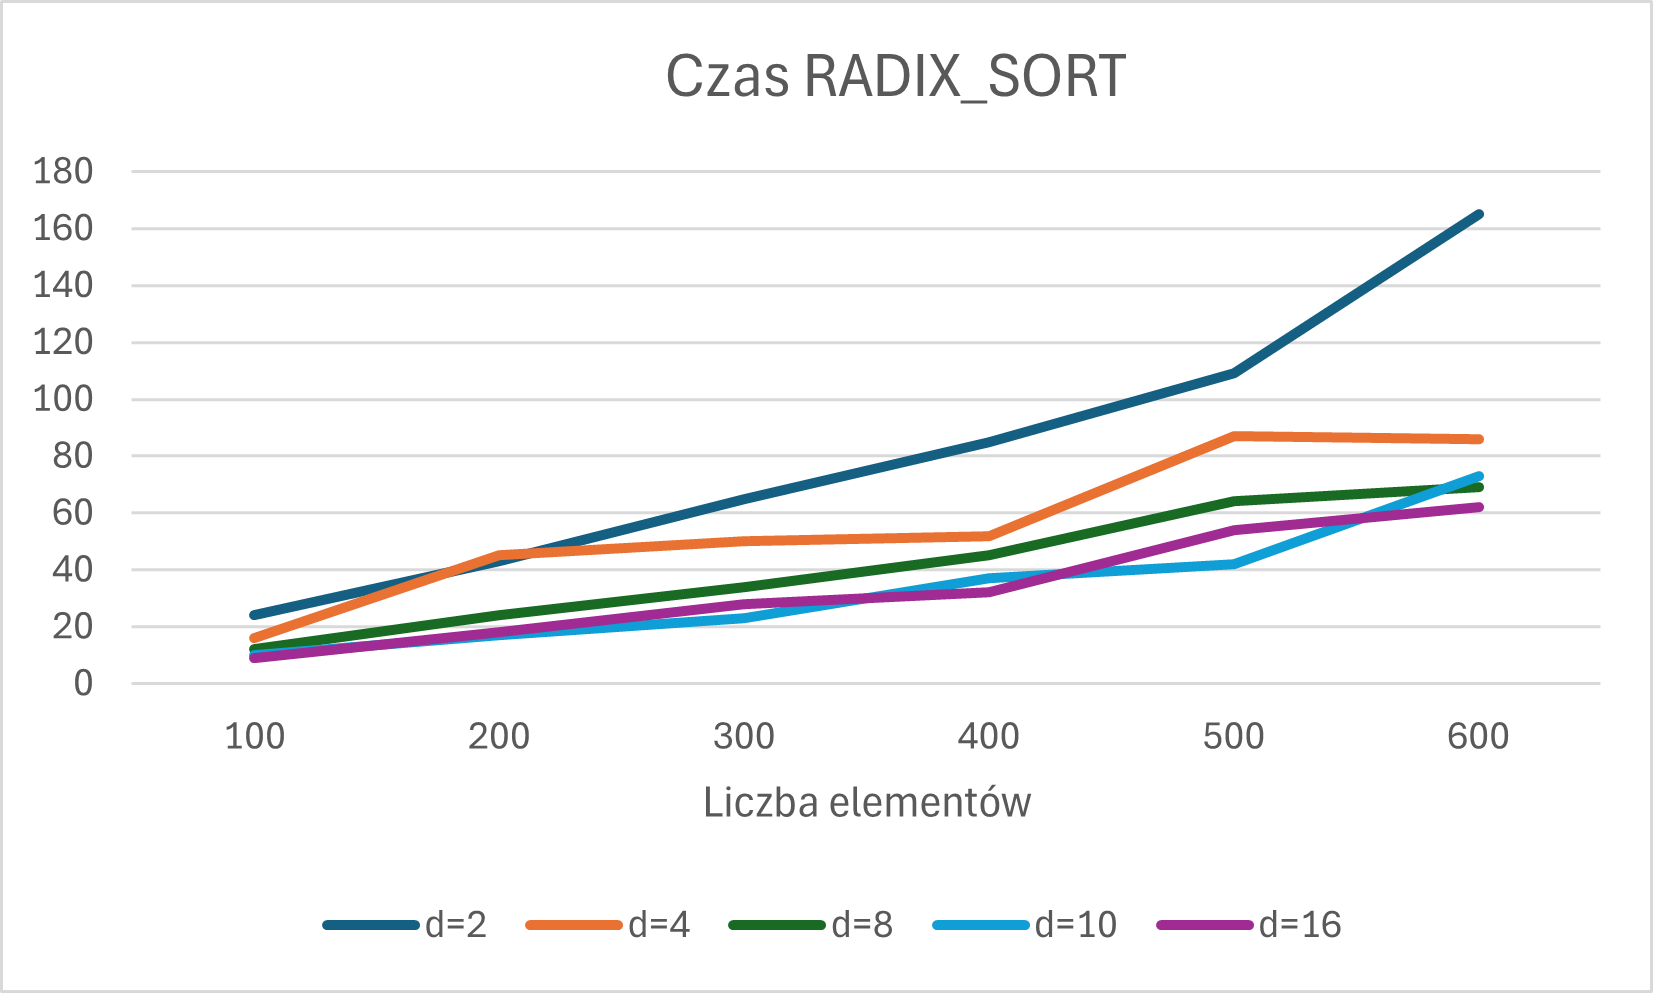
\includegraphics[width=0.9\textwidth]{RS12.png}
		\end{figure}
		
		Liczba przypisań i porównań:
		
		\begin{itemize}
			\item Liczba przypisań rośnie praktycznie liniowo wraz ze wzrostem liczby elementów \( n \).
			\item Zwiększenie podstawy \( d \) (systemu liczbowego) zmniejsza liczbę przypisań, ponieważ mniej iteracji jest potrzebnych do przetworzenia elementów.
			\item Dla \( d = 16 \), liczba przypisań jest praktycznie najmniejsza, podczas gdy dla \( d = 2 \) — największa.
		\end{itemize}
		
		Czas wykonania:
		
		\begin{itemize}
			\item Czas sortowania generalnie zmniejsza się wraz ze wzrostem podstawy \( d \).
			\item Dla większych \( d \), liczba iteracji w głównej pętli algorytmu jest mniejsza, co prowadzi do oszczędności czasu, mimo że pojedynczy krok może mieć większy narzut obliczeniowy.
		\end{itemize}
		
		Efektywność dla różnych podstaw:
		
		\begin{itemize}
			\item Podstawy \( d = 8 \), \( d = 10 \), i \( d = 16 \) wydają się najbardziej efektywne zarówno pod względem liczby przypisań, jak i czasu wykonania.
			\item Dla \( d = 2 \), algorytm wykonuje znacząco więcej operacji, co czyni go najmniej efektywnym.
		\end{itemize}
		\begin{lstlisting}[language=C++, tabsize=3]
	void RADIX_SORT2(int A[], int n, int d, int k) {
		int liczba_dodatnich = 0, liczba_ujemnych = 0;
		
		for (int i = 0; i < n; i++) {
			if (A[i] >= 0) {
				liczba_dodatnich++;
			} else {
				liczba_ujemnych++;
			}
		}
		
		int dodatnie[liczba_dodatnich];
		int ujemne[liczba_ujemnych];
		
		int dod = 0, uje = 0;
		for (int i = 0; i < n; i++) {
			if (A[i] >= 0) {
				dodatnie[dod++] = A[i];
			} else {
				ujemne[uje++] = -A[i]; 
			}
			
			if (liczba_dodatnich > 0) {
				RADIX_SORT(dodatnie, liczba_dodatnich, d, k);
			}
			
			if (liczba_ujemnych > 0) {
				RADIX_SORT(ujemne, liczba_ujemnych, d, k);
			}
			
			int x = 0;
			
			for (int i = liczba_ujemnych - 1; i >= 0; i--) {
				A[x++] = -ujemne[i];
			}
			
			for (int i = 0; i < liczba_dodatnich; i++) {
				A[x++] = dodatnie[i];
			}
		}
			\end{lstlisting}
			
			Działanie funkcji RADIX\_SORT2:
			\begin{itemize}
				\item Zliczanie liczb dodatnich i ujemnych: Funkcja zaczyna od przejścia przez wszystkie elementy tablicy A[], licząc liczbę liczb dodatnich i liczb ujemnych.
				
				\item Inicjalizacja tablic pomocniczych:
				Tworzone są dwie tablice: dodatnie[], ujemne[]. 
				Inicjalizowane są również zmienne dod i uje.
				
				\item Przepisanie liczb do odpowiednich tablic:
				Funkcja przechodzi przez tablicę A[] i, w zależności od znaku liczby, umieszcza ją w odpowiedniej tablicy, ale przed dodaniem każda liczba ujemna jest zmieniana na liczbę dodatnią.
				
				\item Sortowanie obu tablic:
				Jeśli istnieją liczby dodatnie, wywoływana jest funkcja RADIX\_SORT.
				Jeśli istnieją liczby ujemne , wywoływana jest funkcja RADIX\_SORT.
				
				\item Kopiowanie liczb z tablicy ujemnych i dodatnich do oryginalnej tablicy:
				
				Liczby ujemne są kopiowane do tablicy A[] w odwrotnej kolejności, dlatego że liczby ujemne powinny być w porządku malejącym po dodaniu minusa. Następnie liczby dodatnie są kopiowane do tablicy A[] w kolejności rosnącej.
			\end{itemize}
			
			\begin{figure}[H]
				\centering
				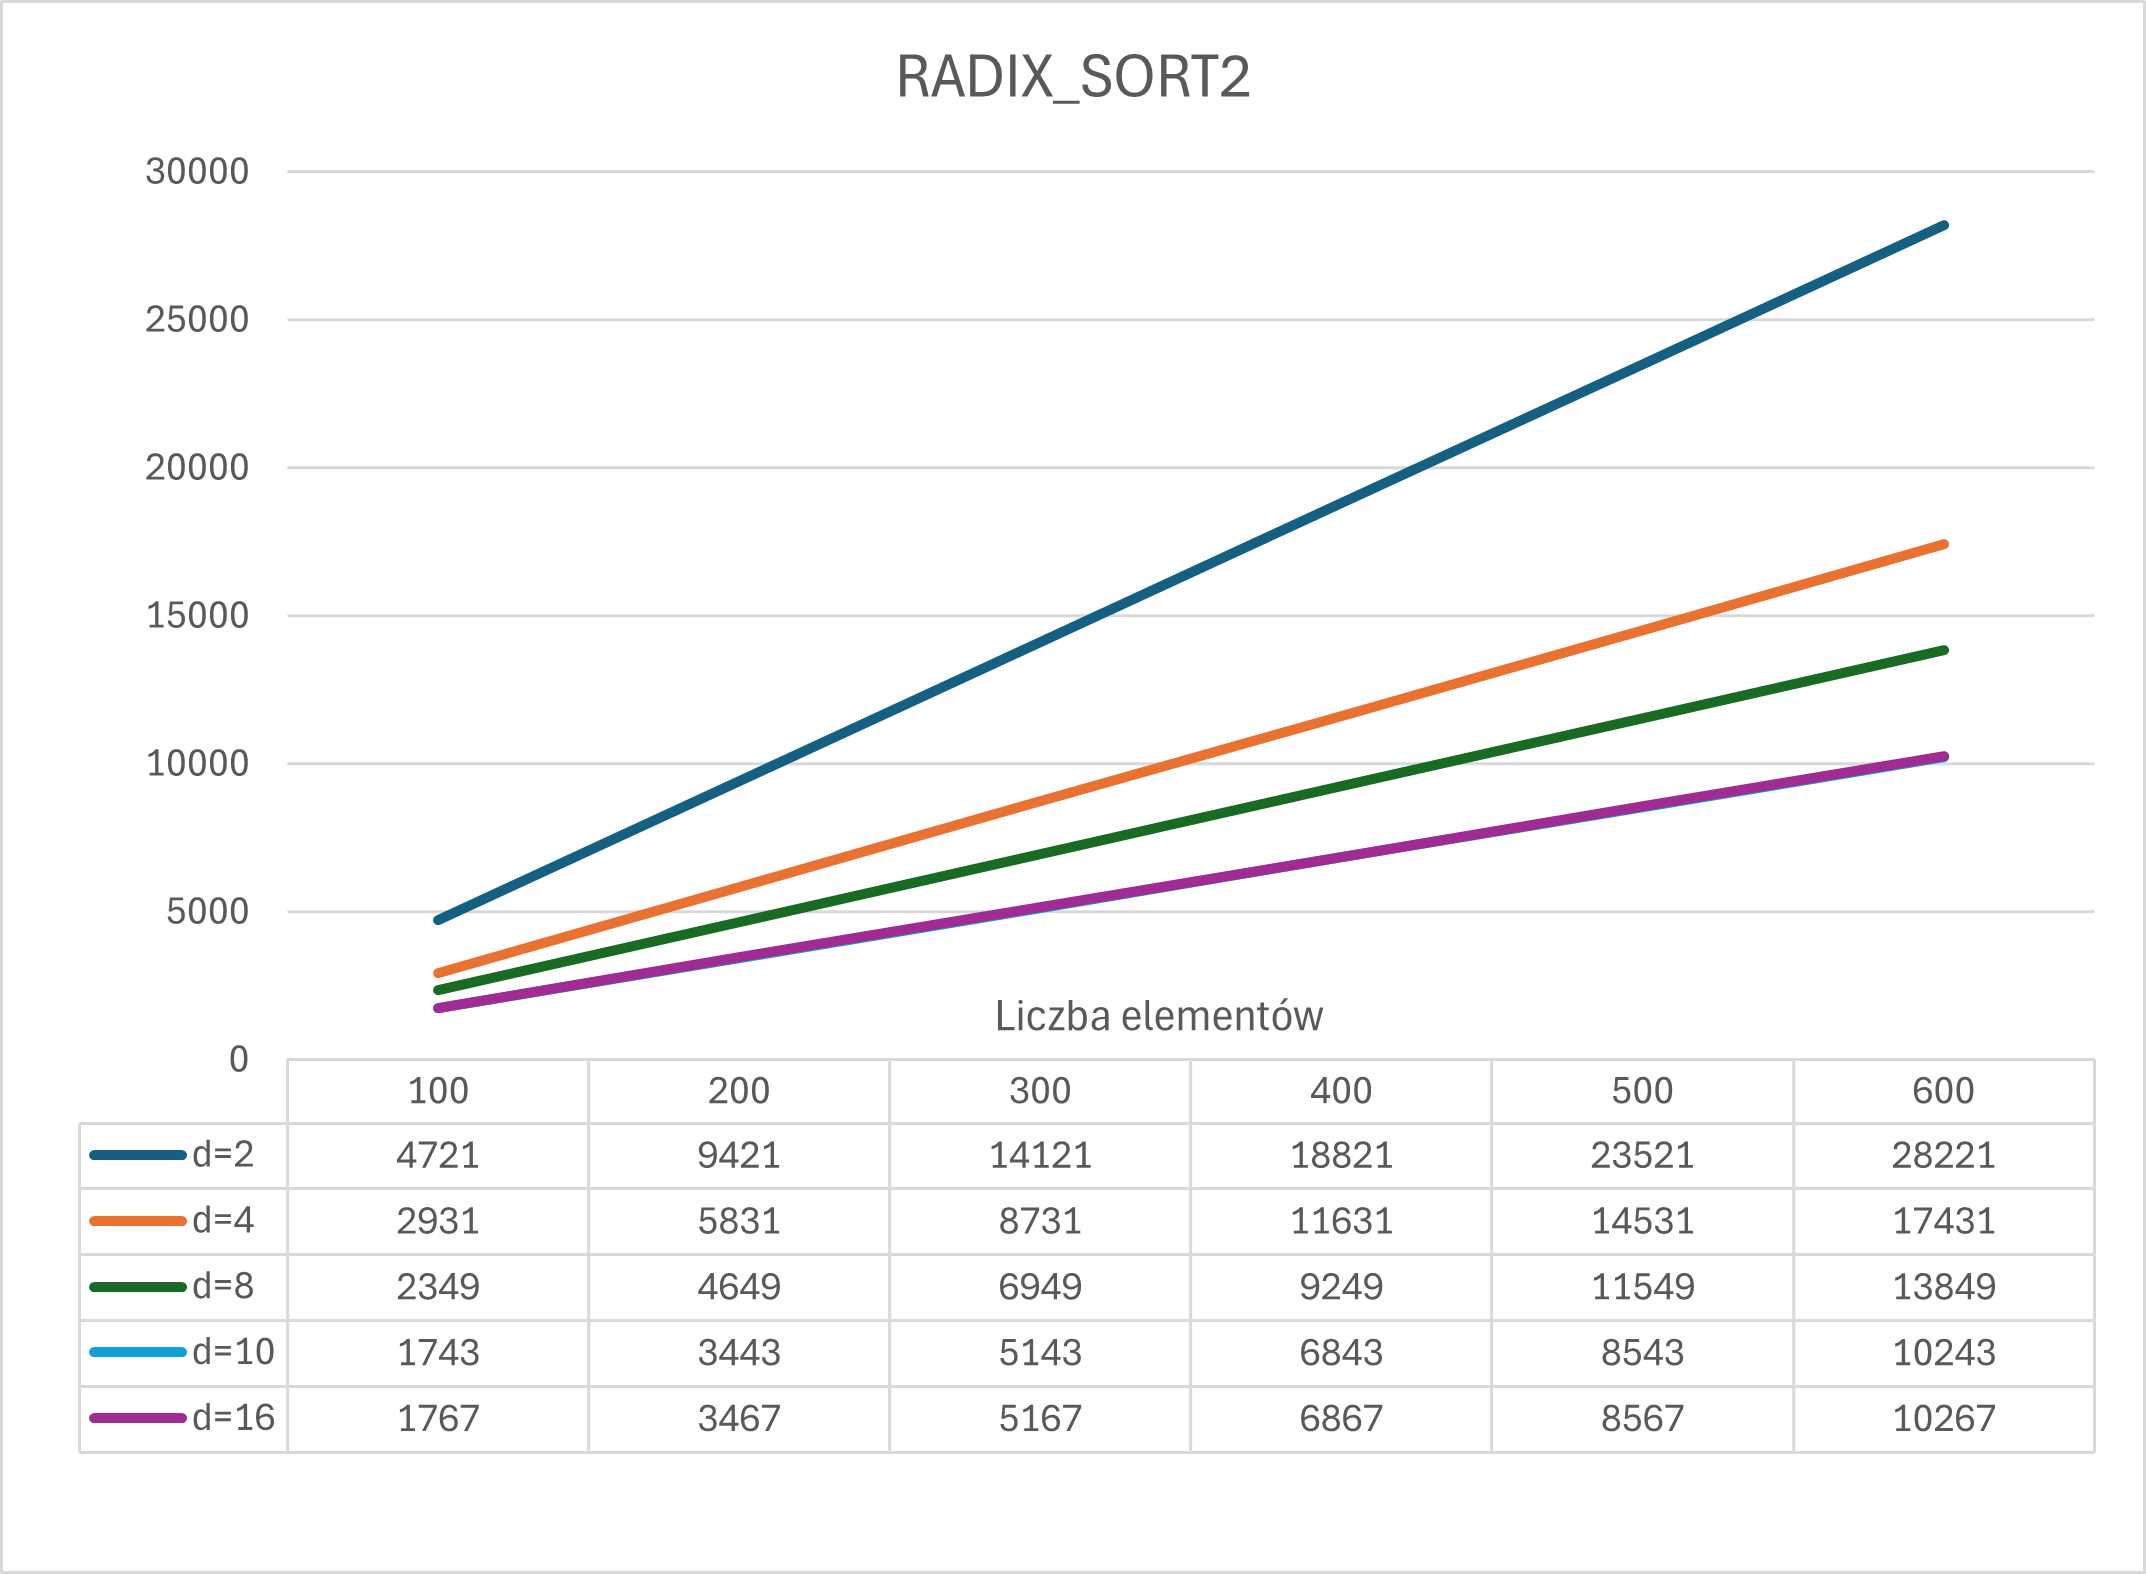
\includegraphics[width=0.9\textwidth]{RS21.png}
				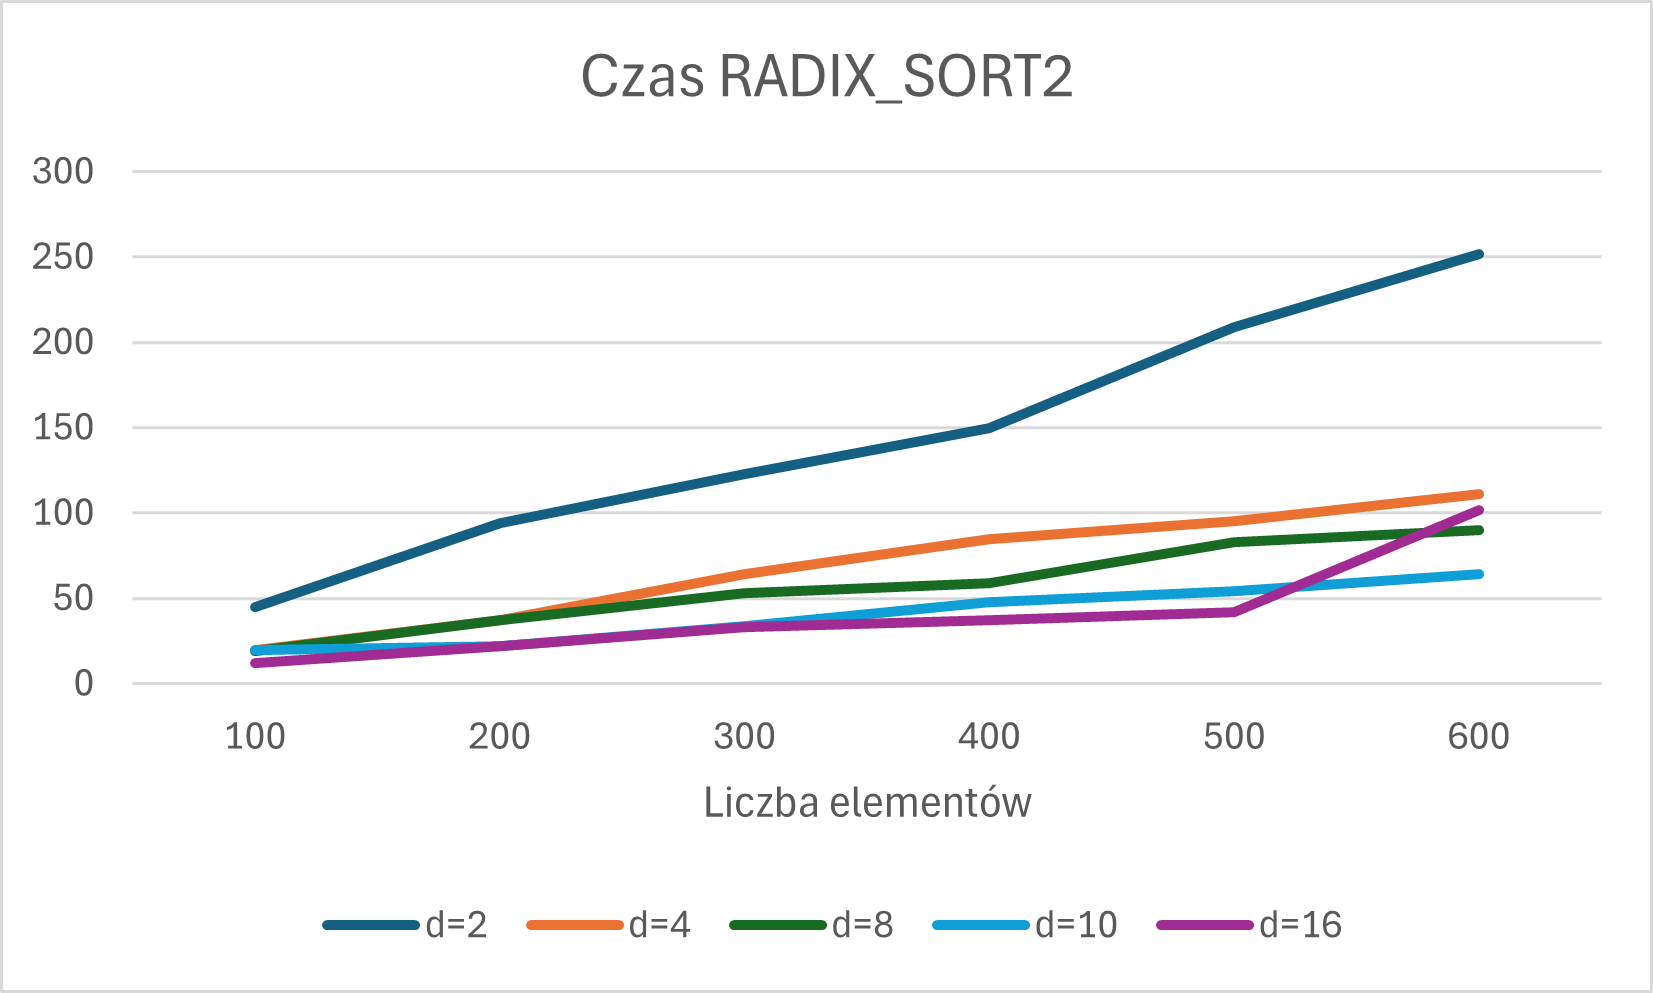
\includegraphics[width=0.9\textwidth]{RS22.png}
			\end{figure}
			
			Liczba przypisań i porównań:
			
			\begin{itemize}
				\item Liczba przypisań rośnie prawie liniowo wraz ze wzrostem liczby elementów \( n \).
				\item Większa podstawa \( d \) zmniejsza liczbę przypisań, ponieważ liczba iteracji algorytmu spada. Najmniej przypisań występuje dla \( d = 16 \) i \( d = 10 \), a najwięcej dla \( d = 2 \).
			\end{itemize}
			
			Czas wykonania:
			
			\begin{itemize}
				\item Czas działania maleje wraz ze wzrostem podstawy \( d \), ponieważ większe \( d \) oznacza mniej iteracji w algorytmie.
				\item Dla \( d = 16 \) i \( d = 10 \), algorytm osiąga najlepsze wyniki czasowe, podczas gdy dla \( d = 2 \) działa najwolniej.
			\end{itemize}
			
			Efektywność dla różnych podstaw:
			
			\begin{itemize}
				\item Podstawy \( d = 8 \), \( d = 10 \), i \( d = 16 \) zapewniają dobrą równowagę między liczbą przypisań a czasem wykonania.
				\item Obsługa ujemnych liczb jest skuteczna dzięki rozdzieleniu ich od dodatnich i niezależnemu sortowaniu.
			\end{itemize}
			
			\newpage
			\section*{Zadanie 3}
			
			\begin{lstlisting}[language=C++, tabsize=3] 
	struct Wezel {
		double wartosc;     
		Wezel* prev;  
		Wezel* next; 
		
		Wezel(double war) : wartosc(war), prev(nullptr), next(nullptr) {} 
	};
	
	struct Lista {
		Wezel* head;
		
		Lista() : head(nullptr) {} 
	};
			\end{lstlisting}
			
			Struktura Wezel reprezentuje pojedynczy element listy. Każdy węzeł zawiera trzy składowe:
			\begin{itemize}
				\item wartosc (typ double):	Przechowuje wartość przechowywaną w danym węźle listy. 
				\item prev (typ Wezel*): Wskaźnik do poprzedniego węzła w liście.
				\item next (typ Wezel*): Wskaźnik do następnego węzła w liście.
				\item Konstruktor Wezel(double war): Jest to konstruktor, który przyjmuje wartość typu double i ustawia ją jako wartość węzła (wartosc). Ponadto, wskaźniki prev i next są inicjalizowane jako nullptr, ponieważ na początku węzeł nie jest połączony z żadnym innym węzłem.
			\end{itemize}
			
			Struktura Lista reprezentuje całą listę. Zawiera ona tylko jedną składową:
			\begin{itemize}
				\item head (typ Wezel*): Jest to wskaźnik do pierwszego węzła w liście. Jeśli lista jest pusta, head jest ustawiony na nullptr. 
				
				\item Konstruktor Lista(): Jest to konstruktor, który inicjalizuje wskaźnik head jako nullptr. Początkowo lista jest pusta, ponieważ nie ma żadnych węzłów.
			\end{itemize}
			
			\begin{lstlisting}[language=C++, tabsize=3] 
	void LIST_INSERT(Lista& L, Wezel* x) {
		x->next = L.head;
		x->prev = nullptr; 
		
		if (L.head != nullptr) {
			L.head->prev = x;
		}
		L.head = x;
	}
	
	void LIST_DELETE(Lista& L, Wezel* x) {
		if (x->prev != nullptr) {
			x->prev->next = x->next;
		} else {
			L.head = x->next; 
		}
		
		if (x->next != nullptr) {
			x->next->prev = x->prev;
		}
		
		delete x; 
	}
	
	Wezel* LIST_SEARCH(Lista& L, double k) {
		Wezel* x = L.head;
		
		while (x != nullptr && x->wartosc != k) {
			x = x->next;
		}
		
		return x; 
	}
	
	void PRINT_LIST(Lista& L) {
		Wezel* x = L.head;
		while (x != nullptr) {
			cout << x->wartosc << " ";
			x = x->next;
		}
		cout << endl;
	}
			\end{lstlisting}
			
			\subsubsection*{1. LIST\_INSERT(Lista\& L, Wezel\* x)}
			
			Ta funkcja wstawia nowy węzeł \texttt{x} na początek listy \texttt{L}.
			\begin{itemize}
				\item Ustawia \texttt{x->next} na dotychczasową głowę listy (\texttt{L.head}), a \texttt{x->prev} na \texttt{nullptr}.
				\item Jeśli lista nie jest pusta (\texttt{L.head != nullptr}), aktualizuje wskaźnik \texttt{L.head->prev} na \texttt{x}.
				\item Ustawia \texttt{L.head} na \texttt{x}, który staje się nowym pierwszym węzłem.
			\end{itemize}
			
			\subsubsection*{2. LIST\_DELETE(Lista\& L, Wezel\* x)}
			
			Ta funkcja usuwa węzeł \texttt{x} z listy \texttt{L}.
			\begin{itemize}
				\item Jeśli \texttt{x} nie jest pierwszym węzłem (\texttt{x->prev != nullptr}), aktualizuje wskaźnik \texttt{x->prev->next} na \texttt{x->next}.
				\item Jeśli \texttt{x} jest pierwszym węzłem (\texttt{x->prev == nullptr}), aktualizuje \texttt{L.head} na \texttt{x->next}.
				\item Jeśli \texttt{x->next != nullptr}, aktualizuje wskaźnik \texttt{x->next->prev} na \texttt{x->prev}.
				\item Na końcu usuwa węzeł \texttt{x} za pomocą \texttt{delete}.
			\end{itemize}
			
			\subsubsection*{3. LIST\_SEARCH(Lista\& L, double k)}
			
			Funkcja ta przeszukuje listę \texttt{L} w poszukiwaniu węzła o wartości \texttt{k}.
			\begin{itemize}
				\item Zaczyna od \texttt{L.head} i przechodzi przez kolejne węzły, porównując ich wartość z \texttt{k}.
				\item Jeśli znajdzie węzeł o wartości \texttt{k}, zwraca wskaźnik do niego.
				\item Jeśli nie znajdzie takiego węzła, zwraca \texttt{nullptr}.
			\end{itemize}
			
			\subsubsection*{4. PRINT\_LIST(Lista\& L)}
			
			Funkcja ta wypisuje wszystkie wartości w liście \texttt{L} w kolejności od głowy listy do ostatniego węzła.
			\begin{itemize}
				\item Zaczyna od \texttt{L.head} i przechodzi po wszystkich węzłach, wypisując ich wartości.
				\item Po wypisaniu wszystkich wartości, wypisuje znak nowej linii.
			\end{itemize}
			
			\subsubsection*{5. INSERTION\_SORT(Lista\& L)}
			\begin{lstlisting}[language=C++, tabsize=3] 
	void INSERTION_SORT(Lista& L) {
		if (L.head == nullptr || L.head->next == nullptr) {
			return; 
		}
		
		Wezel* x = L.head->next; 
		while (x != nullptr) {
			Wezel* Key = x;
			Wezel* prevKey = x->prev;
			
			while (prevKey != nullptr && prevKey->wartosc > Key->wartosc) {
				swap(prevKey->wartosc, Key->wartosc);
				Key = prevKey;
				prevKey = prevKey->prev;
			}
			
			x = x->next;
		}
	}
			\end{lstlisting}
			
			\begin{itemize}
				\item Funkcja rozpoczyna działanie od sprawdzenia, czy lista jest pusta lub zawiera tylko jeden element. W takim przypadku sortowanie nie jest potrzebne i funkcja kończy działanie.
				\item Następnie, funkcja ustawia wskaźnik \texttt{x} na drugi węzeł listy, ponieważ pierwszy węzeł uznawany jest za "posortowany" w kontekście tego algorytmu.
				\item Dla każdego węzła na liście, funkcja porównuje jego wartość z wartością poprzednich węzłów. Jeśli wartość bieżącego węzła jest mniejsza niż wartość poprzedniego, element jest przesuwany do odpowiedniej pozycji w "posortowanej części" listy.
				\item Wstawianie elementu polega na iteracyjnym porównywaniu i zamienianiu wartości węzłów, aż element znajdzie swoje miejsce w posortowanej części listy.
				\item Proces ten powtarza się dla wszystkich węzłów w liście, aż cała lista zostanie posortowana.
			\end{itemize}
			
			\begin{figure}[H]
				\centering
				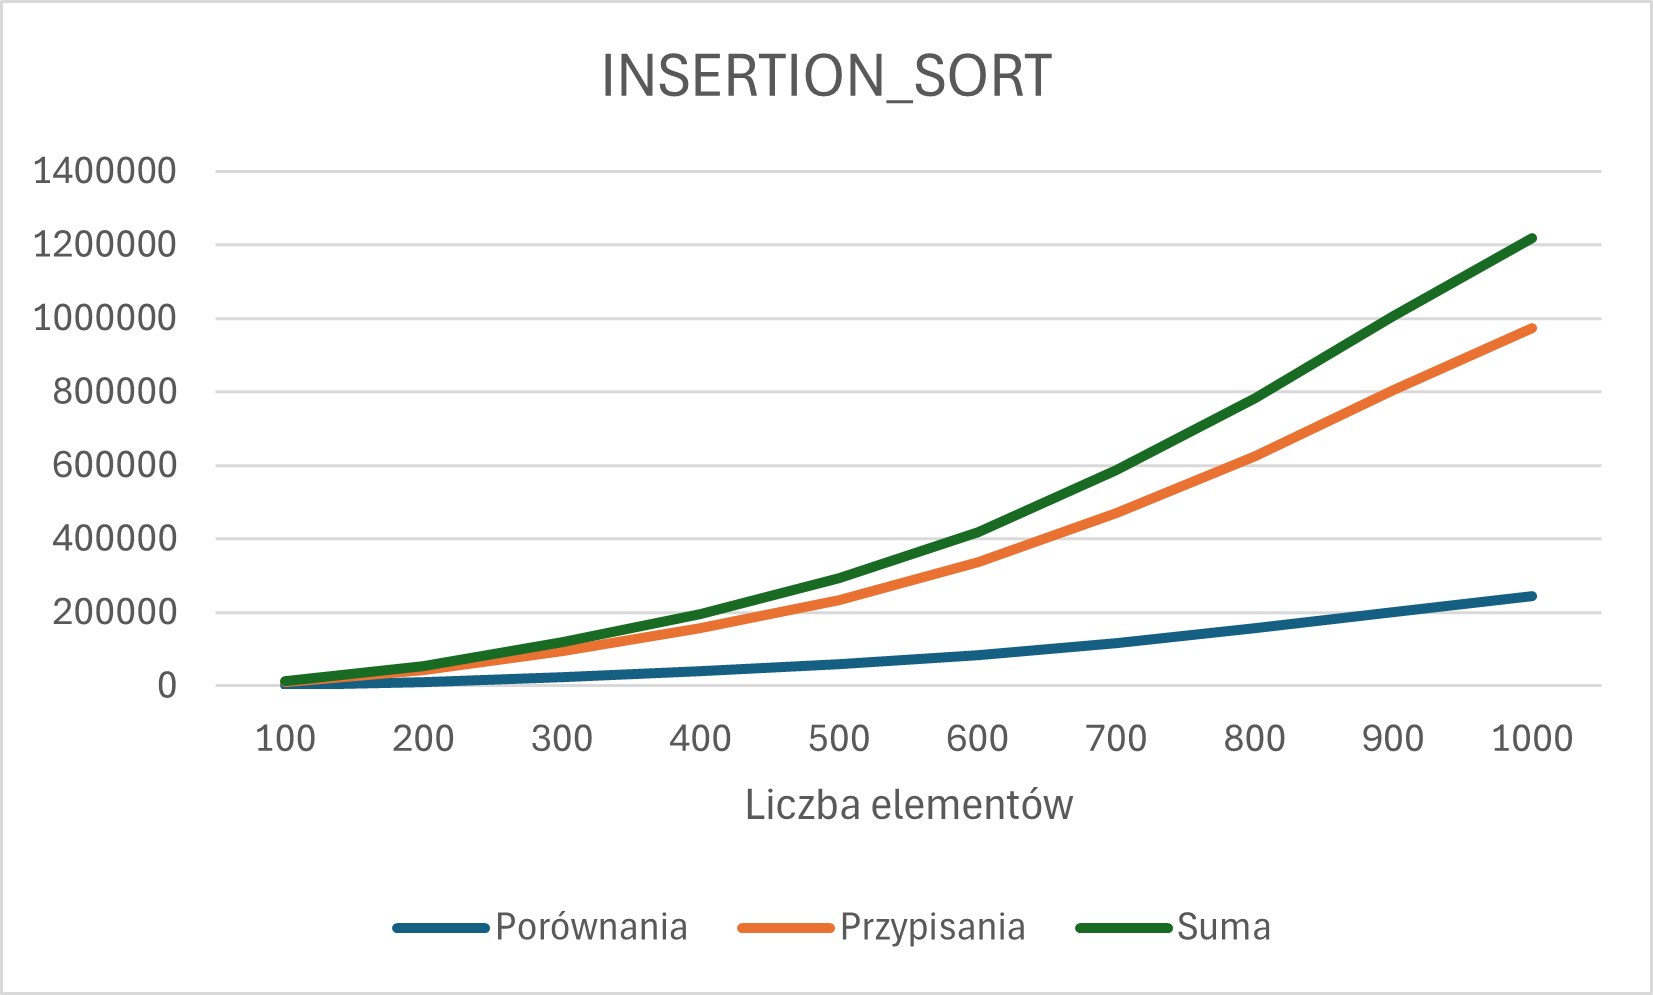
\includegraphics[width=0.9\textwidth]{IS1.png}
				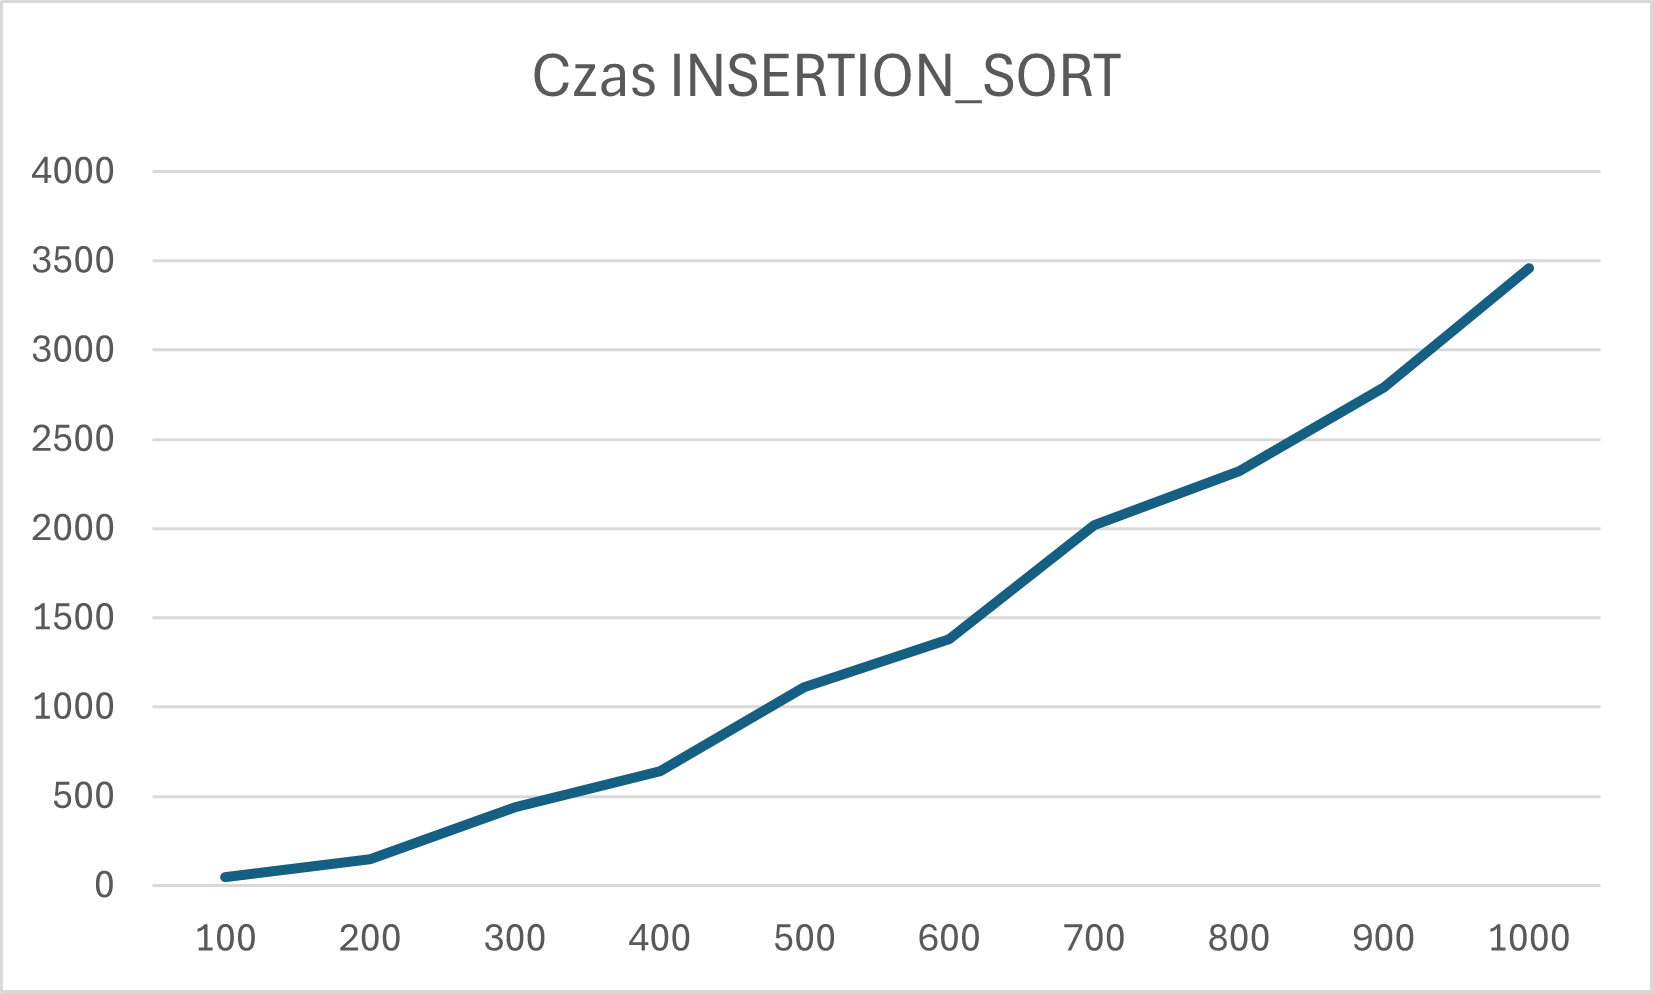
\includegraphics[width=0.9\textwidth]{IS2.png}
			\end{figure}
			
			Funkcja insertion ma rosnący czas wykonania w miarę zwiększania liczby elementów. Czas rośnie nieliniowo, szczególnie dla większej liczby elementów. Wraz ze wzrostem liczby elementów rośnie liczba porównań i przypisań.
			
			\newpage
			\section*{Zadanie 4}
			
			\begin{lstlisting}[language=C++, tabsize=3] 
	void BUCKET_SORT(double A[], int n) {
		Lista B[n]; 
		
		for (int j = 0; j < n; j++) {
			B[j] = Lista();
		}
		
		for (int i = 0; i < n; i++) {
			int index = static_cast<int>(n * A[i]); 
			Wezel* nowy = new Wezel(A[i]);   
			LIST_INSERT(B[index], nowy);    
		}
		
		for (int j = 0; j < n; j++) {
			INSERTION_SORT(B[j]);
		}
		
		int i = 0;
		for (int j = 0; j < n; j++) {
			Wezel* x = B[j].head;
			while (x != nullptr) {
				A[i++] = x->wartosc; 
				x = x->next;
			}
		}
	}
			\end{lstlisting}
			
			Algorytm \textbf{BUCKET\_SORT} dzieli dane na kilka "kubełków" (ang. \textit{buckets}), sortuje każdy kubełek osobno (. \textit{Insertion Sort}), a następnie łączy posortowane kubełki w jedną posortowaną tablicę.
			
			\begin{enumerate}
				\item \textbf{Inicjalizacja kubełków:}
				Algorytm tworzy tablicę \( B \), która zawiera \( n \) pustych list, reprezentujących kubełki. Każdy kubełek przechowuje elementy, które zostaną przypisane do niego na podstawie wartości z tablicy wejściowej \( A \). Dla każdego kubełka tworzona jest pusta lista.
				
				\item \textbf{Rozdzielanie elementów do kubełków:}
				Każdy element z tablicy \( A \) jest przypisywany do odpowiedniego kubełka na podstawie swojej wartości. Obliczamy indeks kubełka dla każdego elementu \( A[i] \), który zależy od wartości \( A[i] \) oraz liczby kubełków \( n \).
				
				\item \textbf{Sortowanie wewnętrzne kubełków:}
				Po przypisaniu wszystkich elementów do kubełków, każdy kubełek jest sortowany indywidualnie. Ponieważ kubełki zawierają elementy z określonego przedziału, sortowanie w każdym kubełku jest szybkie.
				
				\item \textbf{Łączenie posortowanych kubełków:}
				Po posortowaniu każdego kubełka elementy z kubełków są zbierane i kopiowane z powrotem do tablicy \( A \). Proces ten polega na przejściu przez wszystkie kubełki i przeniesieniu posortowanych elementów z listy węzłów do tablicy wynikowej.
			\end{enumerate}
			
			\begin{figure}[H]
				\centering
				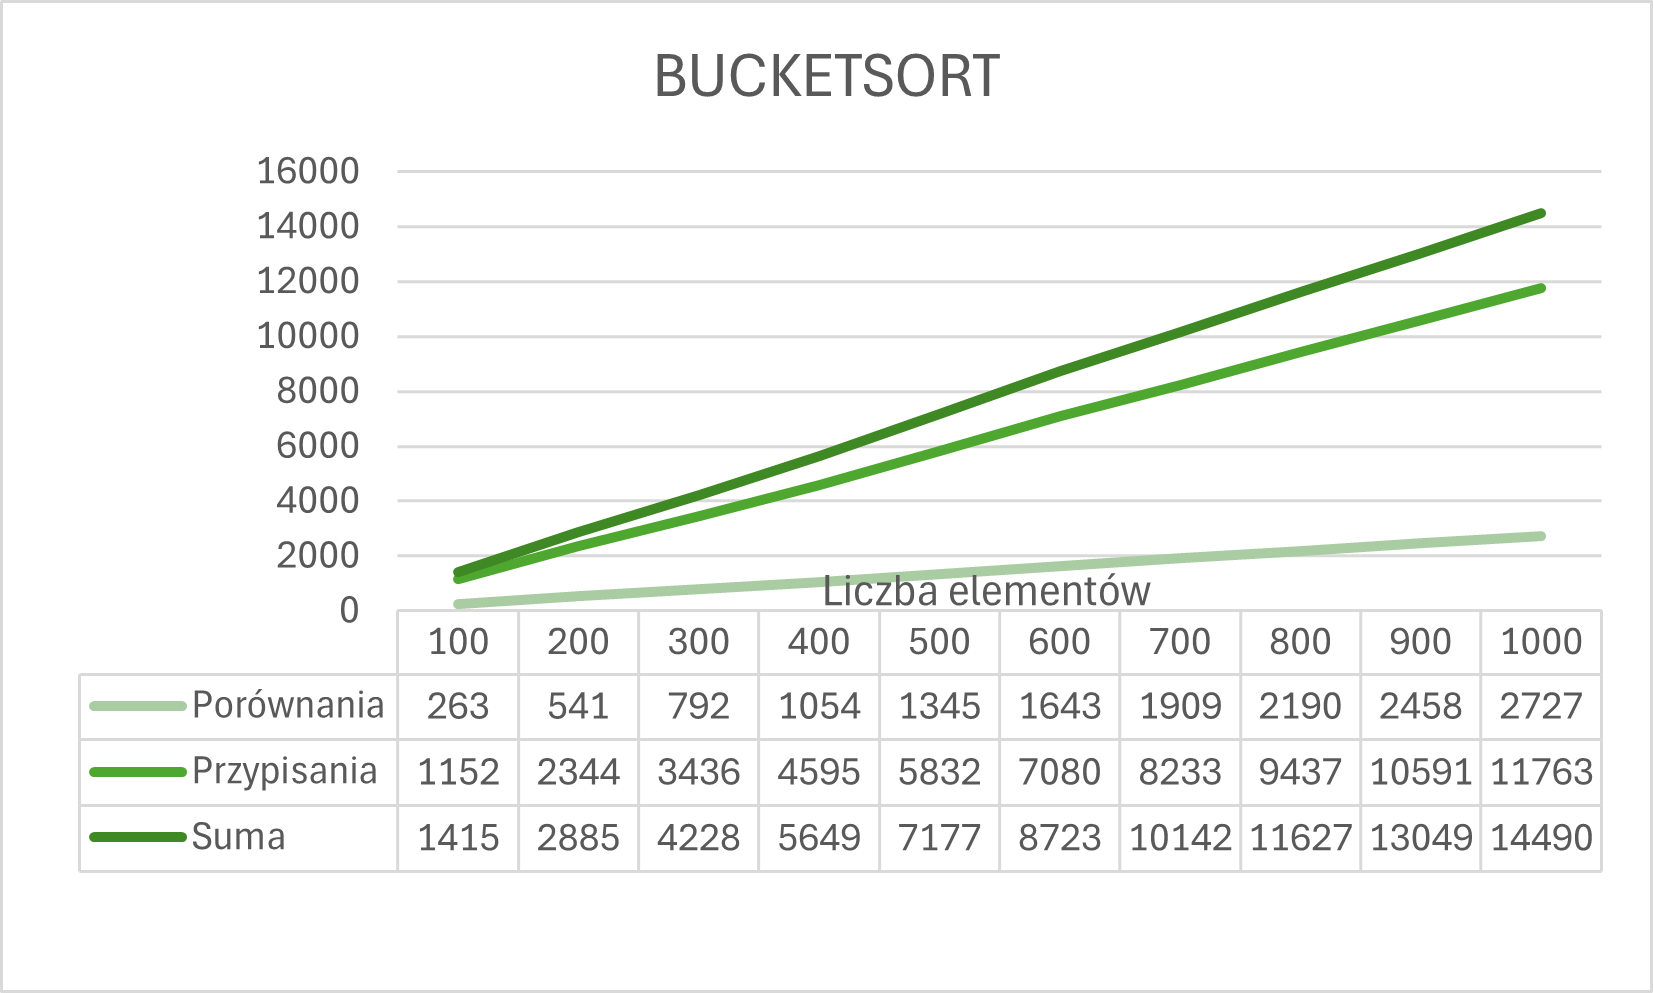
\includegraphics[width=0.9\textwidth]{BS11.png}
				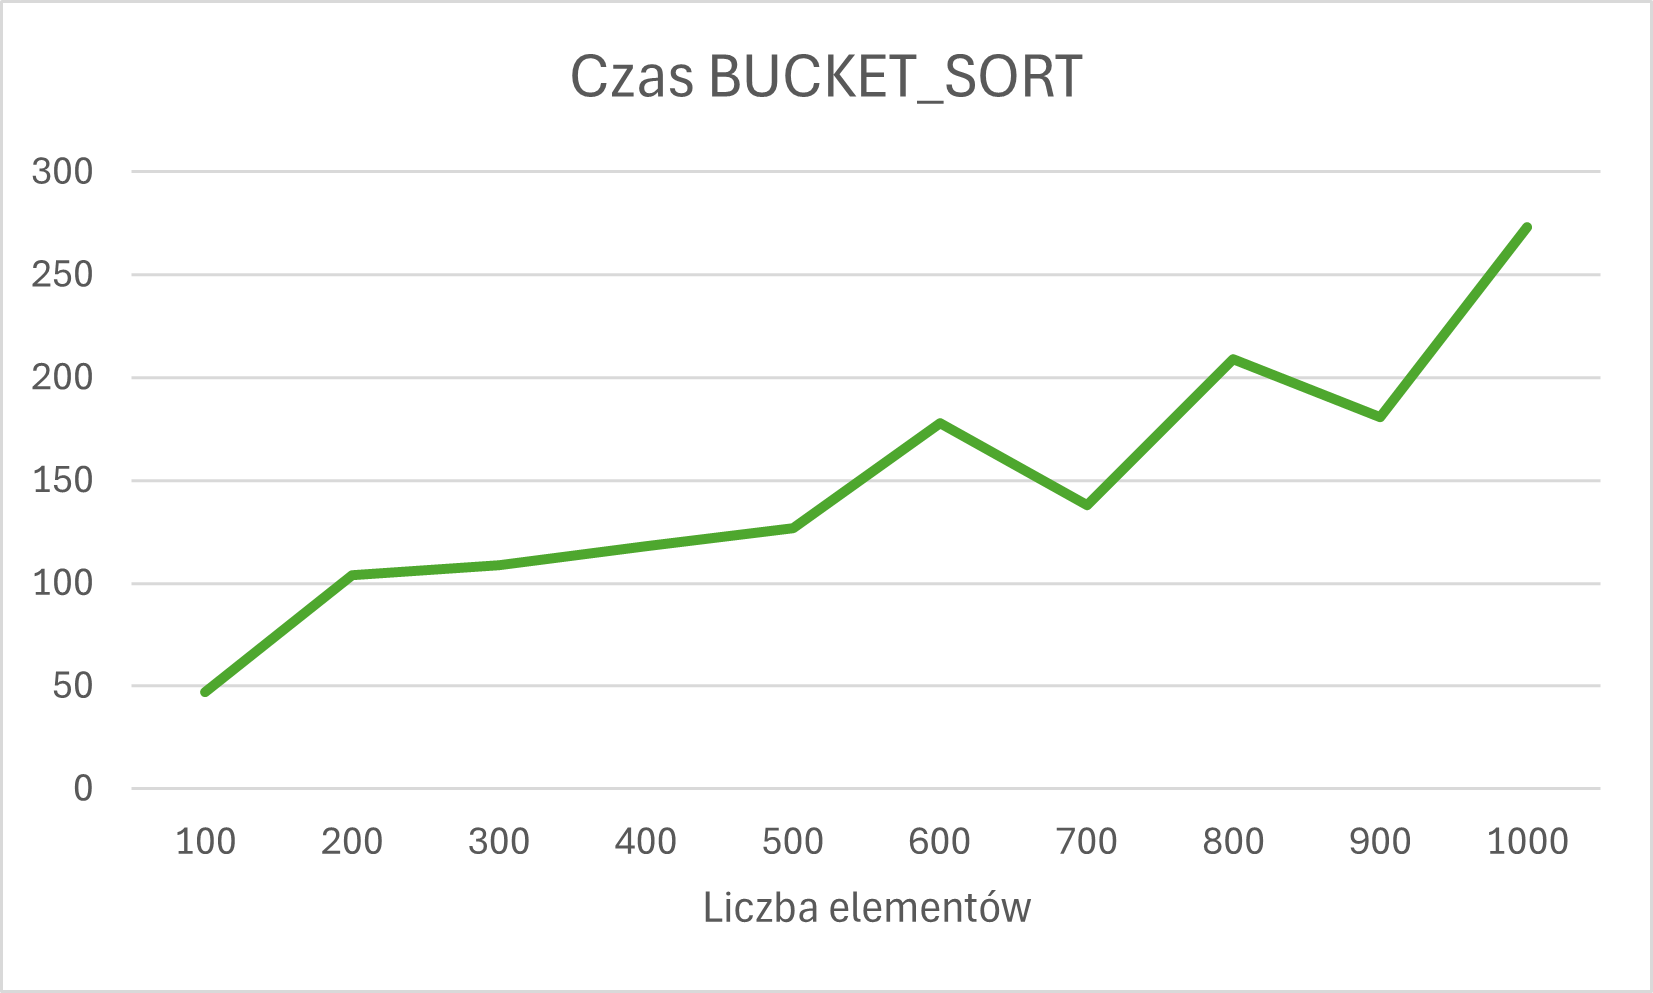
\includegraphics[width=0.9\textwidth]{BS12.png}
			\end{figure}
			
			Algorytm Bucket Sort wykazuje wzrost czasu wykonania oraz liczby operacji (porównań i przypisań) wraz z liczbą elementów. Czas rośnie nieliniowo. Dla mniejszych zbiorów jest stosunkowo szybki, ale dla dużych danych jego wydajność spada, co ogranicza jego zastosowanie przy dużych zbiorach.
			
			\begin{lstlisting}[language=C++, tabsize=3] 
void BUCKET_SORT2(double A[], int n) {
	double minimalna = A[0];
	double maksymalna = A[0];
	for (int i = 1; i < n; i++) {
		if (A[i] < minimalna) minimalna = A[i];
		if (A[i] > maksymalna) maksymalna = A[i];
	}
	
	if (maksymalna == minimalna) {
		for (int i = 0; i < n; i++) {
			A[i] = minimalna; 
		}
		return;
	}
	
	Lista B[n]; 
	
	for (int j = 0; j < n; j++) {
		B[j] = Lista();
	}
	
	for (int i = 0; i < n; i++) {
		int index = static_cast<int>(n*(A[i]-minimalna)/(maksymalna-minimalna)); 
		if (index == n) index--; 
		Wezel* nowy = new Wezel(A[i]);              
		LIST_INSERT(B[index], nowy);                 
	}
	
	for (int j = 0; j < n; j++) {
		INSERTION_SORT(B[j]);
	}
	
	int i = 0;
	for (int j = 0; j < n; j++) {
		Wezel* x = B[j].head;
		while (x != nullptr) {
			A[i++] = x->wartosc; 
			x = x->next;
		}
	}
}
			\end{lstlisting}
			Algorytm \textbf{BUCKET\_SORT2} działa na zasadzie dzielenia elementów na "kubełki", które są następnie sortowane indywidualnie, a następnie scalane w jedną posortowaną tablicę.
			
			\begin{enumerate}
				\item \textbf{Znalezienie minimalnej i maksymalnej wartości w tablicy \( A \):}
				\begin{itemize}
					\item Algorytm rozpoczyna od obliczenia minimalnej i maksymalnej wartości w tablicy \( A \). Te wartości będą potrzebne do prawidłowego rozdzielenia elementów na kubełki.
				\end{itemize}
				
				\item \textbf{Inicjalizacja kubełków:}
				\begin{itemize}
					\item Tworzymy tablicę kubełków \( B \), która składa się z \( n \) pustych list.
				\end{itemize}
				
				\item \textbf{Rozdzielanie elementów do kubełków:}
				\begin{itemize}
					\item Dla każdego elementu \( A[i] \) z tablicy \( A \) obliczamy indeks kubełka, do którego należy go przypisać.
					\item Indeks kubełka obliczany jest na podstawie wzoru:
					\[
					\text{index} = \left\lfloor n \cdot \frac{A[i] - \text{minimalna}}{\text{maksymalna} - \text{minimalna}} \right\rfloor
					\]
					\item Indeks kubełka jest liczony jako liczba całkowita z zakresu od 0 do \( n-1 \), co pozwala na odpowiednie przypisanie elementów do kubełków.
					\item Jeśli indeks wynosi \( n \) (np. dla wartości równych maksymalnej), zmniejszamy go o 1, aby uniknąć przekroczenia zakresu.
					\item Element \( A[i] \) jest następnie dodawany do odpowiedniego kubełka \( B[\text{index}] \) za pomocą funkcji \texttt{LIST\_INSERT}.
				\end{itemize}
				
				\item \textbf{Sortowanie kubełków:}
				\begin{itemize}
					\item Po przypisaniu wszystkich elementów do kubełków, każdy kubełek jest sortowany indywidualnie.
					\item Sortowanie odbywa się przy użyciu algorytmu sortowania przez wstawianie (Insertion Sort) na każdej z list w kubełkach.
				\end{itemize}
				
				\item \textbf{Łączenie posortowanych kubełków:}
				\begin{itemize}
					\item Po posortowaniu kubełków algorytm łączy posortowane elementy z każdego kubełka z powrotem do tablicy \( A \).
				\end{itemize}
			\end{enumerate}
			
			\begin{figure}[H]
				\centering
				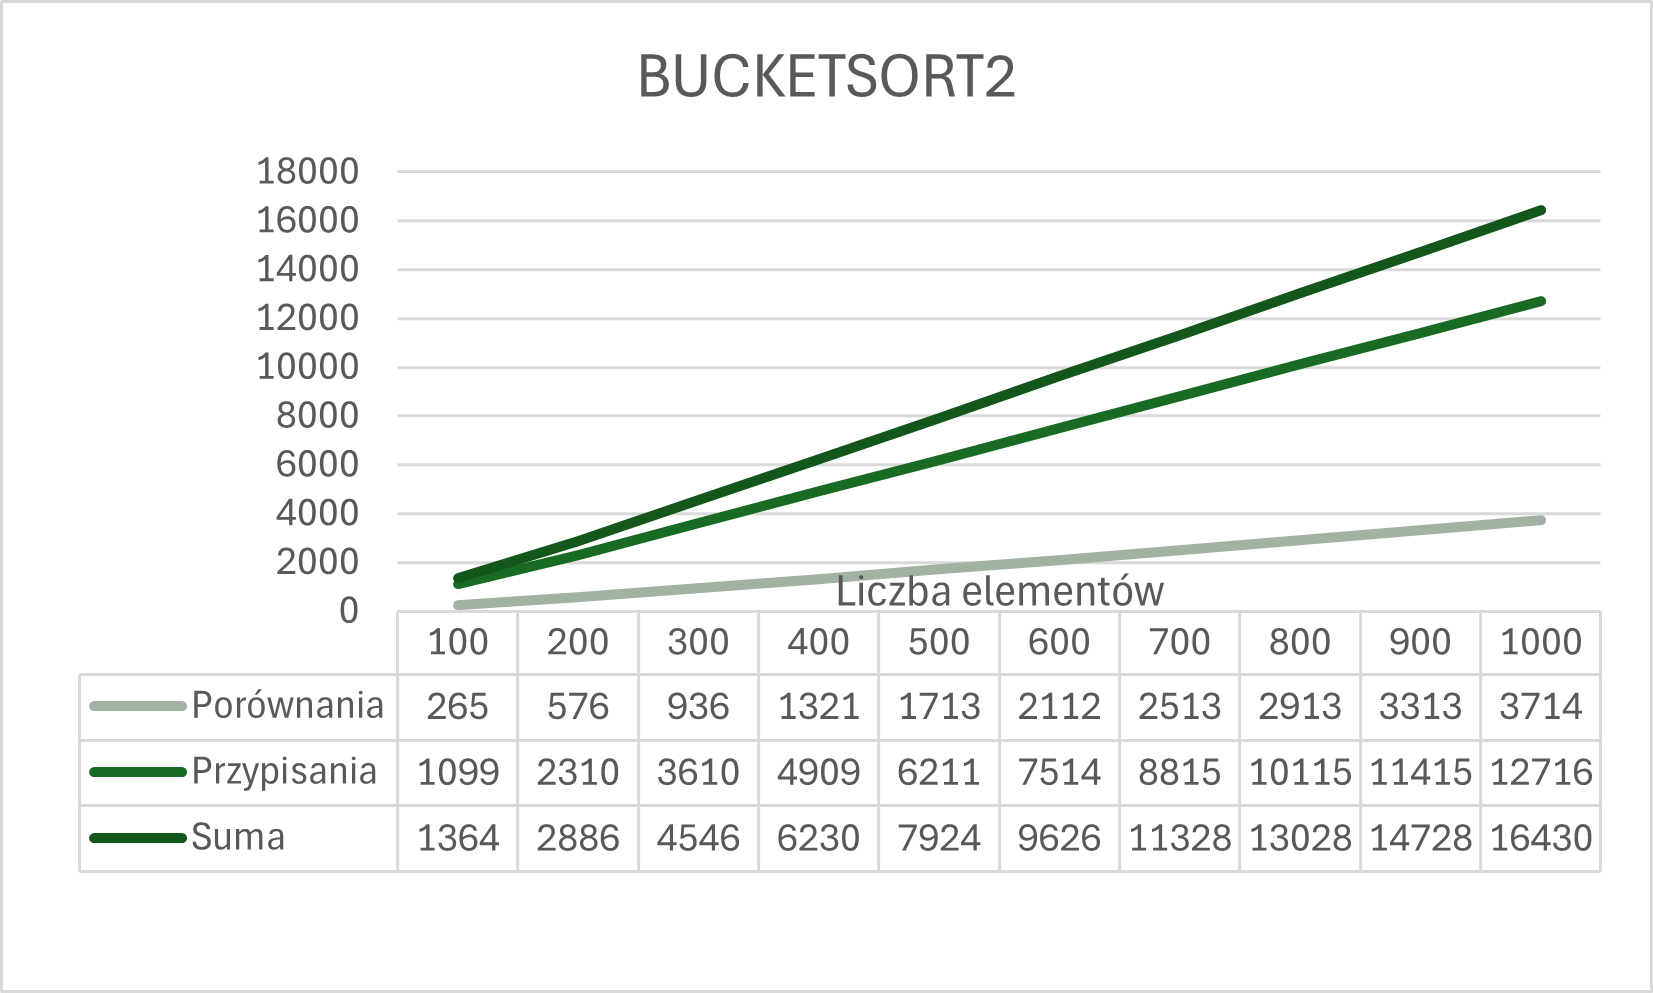
\includegraphics[width=0.9\textwidth]{BS21.png}
				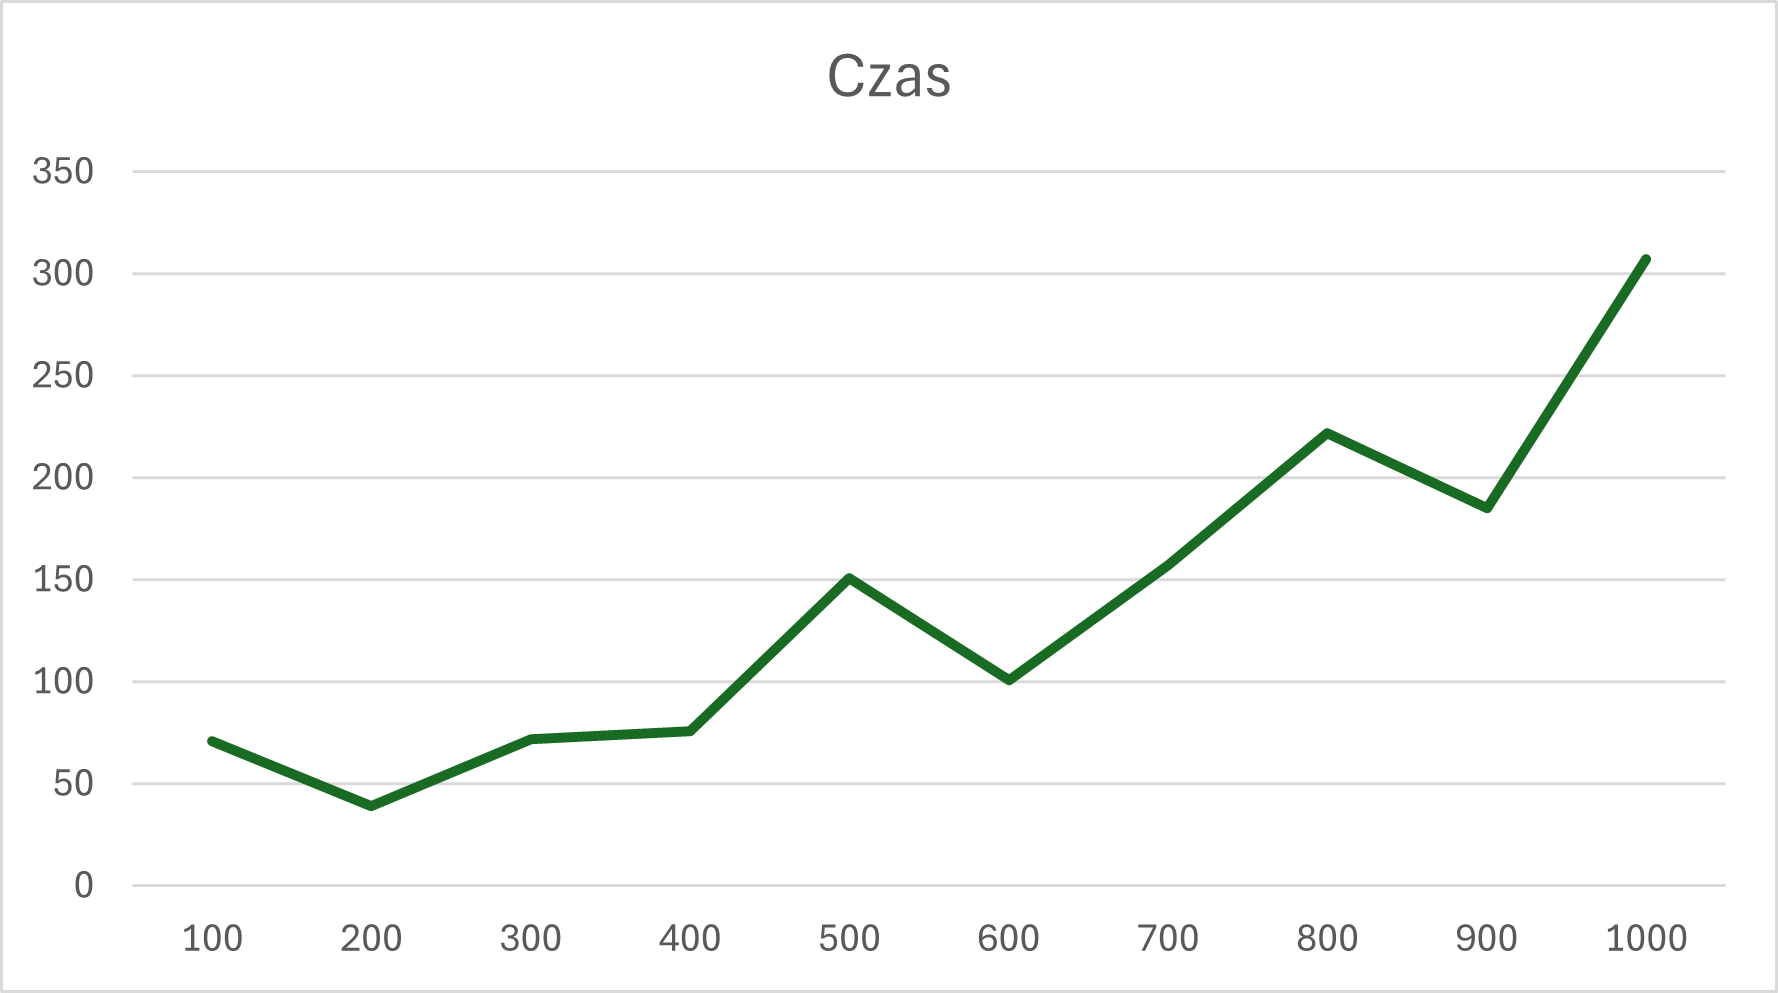
\includegraphics[width=0.9\textwidth]{BS22.png}
			\end{figure}
			
			W Bucket\_Sort2 czas wykonania rośnie nieliniowo z liczbą elementów. Dla małych zbiorów działa efektywnie, jednak przy większych danych czas wykonania i liczba operacji rosną znacząco, co ogranicza jego wydajność przy dużych zbiorach.
			
			\section*{Quick\_Sort i Bucket\_Sort}
			
			\begin{figure}[H]
				\centering
				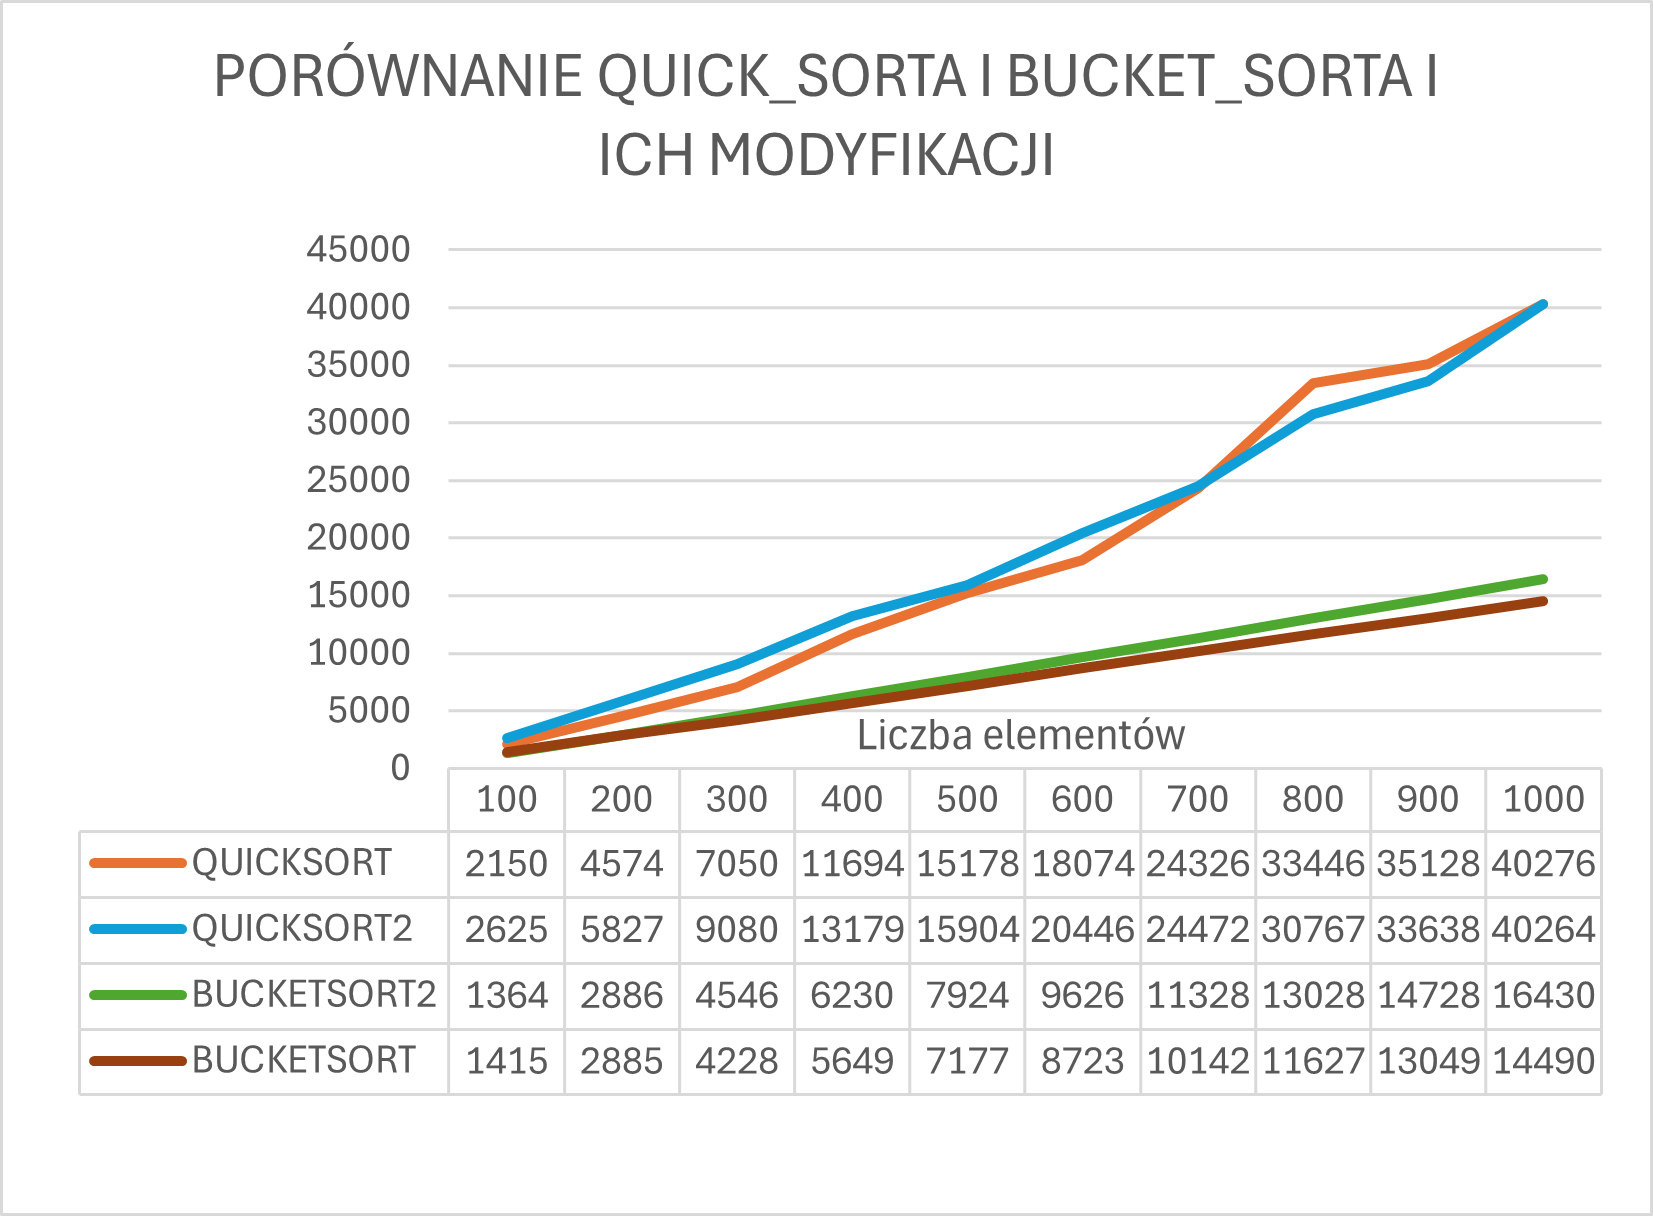
\includegraphics[width=0.9\textwidth]{QSBS1.png}
				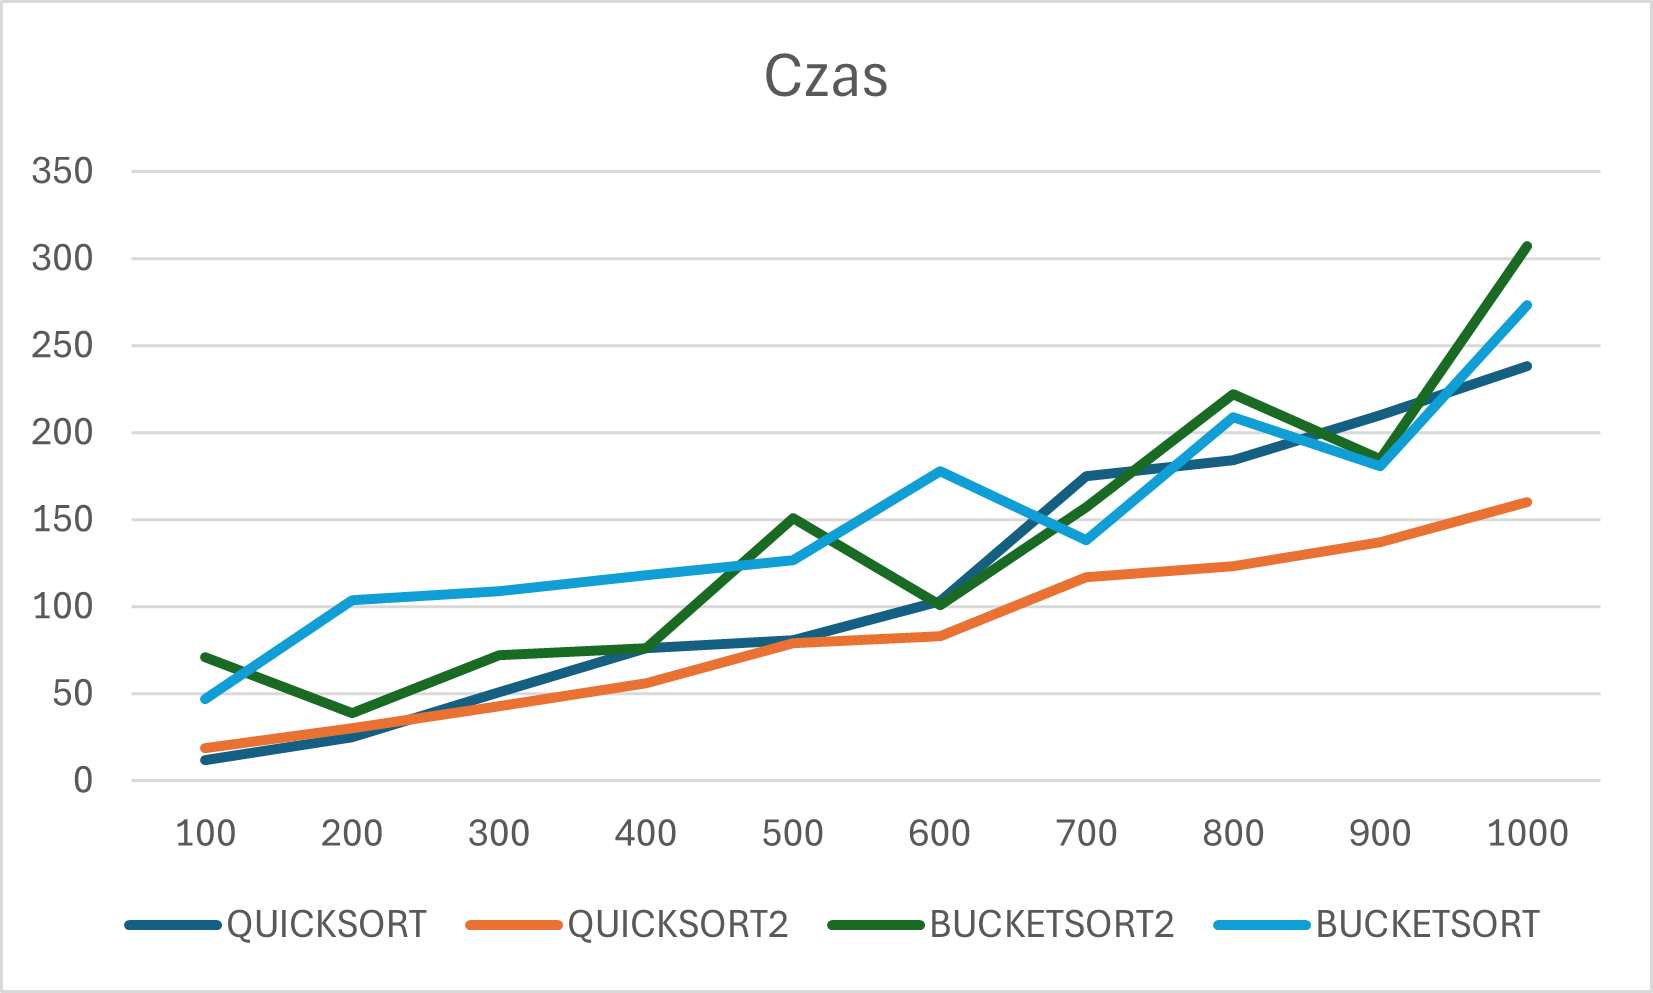
\includegraphics[width=0.9\textwidth]{QSBS2.png}
			\end{figure}
			
			\textbf{Porównania i przypisania:}
			\begin{itemize}
				\item \textbf{BUCKETSORT2} jest najbardziej efektywnym algorytmem pod względem liczby przypisań i porównań dla wszystkich rozmiarów tablic.
				\item \textbf{BUCKETSORT} jest nieznacznie gorszy od \textbf{BUCKETSORT2}, ale nadal bardziej efektywny niż \textbf{QUICKSORT}.
				\item \textbf{QUICKSORT} i \textbf{QUICKSORT2} są do siebie bardzo podobne, a ich wydajność jest gorsza w porównaniu do \textbf{BUCKETSORT} i \textbf{BUCKETSORT2}, szczególnie w przypadku mniejszych dużej ilości elementów.
			\end{itemize}
			
			\textbf{Czas:}
			\begin{itemize}
				\item \textbf{QUICKSORT2} wydaje się być najszybszym algorytmem spośród wszystkich, ponieważ jego czasy wykonania są najniższe w porównaniu do pozostałych algorytmów dla wszystkich rozmiarów tablic.
				\item \textbf{BUCKETSORT} i \textbf{BUCKETSORT2} mają nieregularne czasy wykonania, które rosną z liczbą elementów. Niemniej jednak, ich czas rośnie szybciej niż czas dla \textbf{QUICKSORT2}, szczególnie przy większej liczbie elementów.
				\item \textbf{QUICKSORT} i \textbf{QUICKSORT2} mają stosunkowo regularny wzrost czasów wykonania, jednak \textbf{QUICKSORT2} wypada lepiej pod względem wydajności niż \textbf{QUICKSORT}.
			\end{itemize}
		\end{document}